

\chapter[A comprehensive high-fidelity DMS framework]{A framework for comprehensive and high-fidelity Deep Mutational Scanning}
\label{ch:data1}

The work described below represents a team effort including many members of the Roth Lab. Wet lab elements of the work were performed by Atina Cot\'e, Jennifer Knapp, Song Sun and Marta Verby, while all computational and statistical aspects were developed and implemented by myself, except where indicated otherwise.

\section{Introduction}

% \todo{Cast this introduction more in the light of functional assays and less about disease. (Save that for the next chapter.)}

Deep Mutational Scanning~(DMS)~\cite{fowler_high-resolution_2010,ernst_coevolution_2010,hietpas_experimental_2011}, a strategy for large-scale functional testing of variants, yields functional maps describing a large fraction of substitutions for an often substantial subset of residue positions. The assays used for DMS studies are diverse, often measuring different aspects of a protein's behaviour. Functional complementation assays test a variant's impact on overall protein function by testing the variant gene's ability to rescue the phenotype caused by reduced activity of the wild type gene (or its ortholog in the case of trans-species complementation)~\cite{lee_complementation_1987,osborn_rescuing_2007}. In a previous paper, Song Sun and other members of the Roth Lab have previously found cell-based functional complementation assays to accurately identify disease variants across a diverse collection of human disease genes~\cite{sun_extended_2016}. 

There are many challenges to the DMS strategy.  One challenge is establishment of robust interpretable assays that measure each variant's impact on the disease-relevant functions of a gene. Another is that the fraction of possible amino acid changes that are measured varies from map to map. Finally, many maps do not control for the overall quality of measurements, or estimate the quality of each measurement. The lack of a comprehensively measured map of known-quality functional impact scores limits the opportunity for confident use of DMS maps to evaluate specific variants.

Here, a modular DMS framework will be described to generate complete, high-fidelity maps of variant function based on functional complementation. The framework employs a novel mutagenesis strategy, two alternative sequencing-based selection screens, and a machine learning strategy to impute  otherwise missing parts of the map with surprising accuracy, and uses regularization to correct less confidently measured data points. The framework is evaluated with respect to its performance on the SUMO E2 conjugase \gene{UBE2I}.


\section{Results}

When carrying out deep mutational scans of protein sequences yielding comprehensive atlases of sequence-function relationships, it is useful to describe the process in distinct stages. The framework described in the following sections can be broken down into six such stages (see Figure~\ref{fig:framework}): 1) mutagenesis; 2) generation of a clone library; 3) selection for clones encoding a functional protein; 4) read-out of the selection results and analysis to produce an initial sequence-function map; 5) computational analysis to impute missing values; and 6) computational analysis to refine measured values based on imputation models. The framework incorporates previously-described deep mutational scanning concepts as well as new experimental components (e.g. an imputation and regularization strategy) and analytic methods. In particular, the last two stages enabling a complete and accurate DMS map have not been applied in any published DMS study.

In the following sections, I will first describe a version of the framework called DMS-BarSeq and apply it to the human SUMO conjugase \gene{UBE2I}, exhaustively measuring the ability of protein variants to function. DMS-BarSeq provides direct variant function measurements and the ability to examine higher-order multi-mutant effects. An alternative version of the framework, DMS-TileSeq, generally captures only single-variant effects, but is less resource-intensive. After comparing DMS-TileSeq and DMS-BarSeq, the resulting maps are combined, missing data points are computationally inferred and map quality refined.


\begin{figure}[h!]
	\centering
	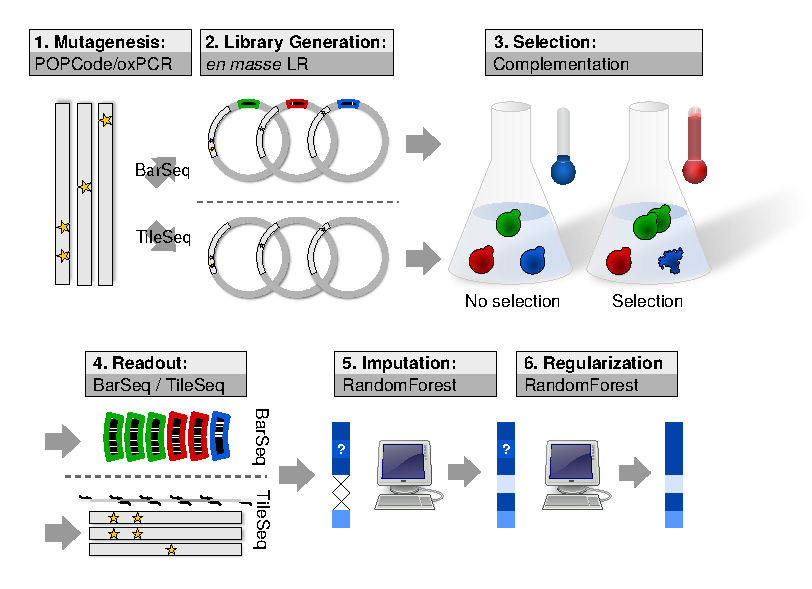
\includegraphics[width=\textwidth]{img/framework_flowchart.pdf}
	\caption{An overview of the Deep Mutational Scanning Framework. Step 1: Using mutagenesis via POPCode and oxidized nucleotide PCR, a pool of variant ORFs is created. Step 2: A library is generated via en-masse gateway cloning. Depending on the downstream sequencing procedure either plain or barcoded expression vectors are used. Step 3: Clones compete with each other for growth under selective and control conditions. Step 4: In case of BarSeq, barcodes are sequenced and counted. In case of TileSeq, individual tiles within the ORF are amplified used in paired-end sequencing. Step 5: Machine Learning methods are used to impute the effects of missing variants. Step 6: Machine learning predictions are also used to support less confidently measured variants. (Incl. illustrations by \cite{kossin_thermometer_2004,bons_computer_2005})}
	\label{fig:framework}
\end{figure}


\subsection{A barcode-based Deep Mutational Scanning strategy}

%Describe goals for this screen, and then how the different choices below aim to achieve these.

As an initial test of the overall framework, we first aimed to generate a map of functional missense variation for \gene{UBE2I}. Our goals for this map were as follows: (i) High and even coverage of the full spectrum of amino acid changes; (ii) Determination of mutant effects on overall protein functionality; (iii) High fidelity of functional effect readouts. We therefore designed the different stages of the framework accordingly. 

For Stage 1 of the DMS-BarSeq framework---mutagenesis---to achieve a relatively even representation of all possible single amino acid substitutions, we wished to allow multiple mutations per clone. This would not only allow for greater mutational coverage for any given library size, but it would also offer an opportunity to discover intragenic epistatic relationships between variants.  To fulfill these requirements, we developed a mutagenesis protocol (Precision Oligo-Pool based Code Alteration or POPCode) which generates random codon replacements. 
At the second stage---library generation---we wished to be able to track the fitness effects of each individual mutant clone rather than just average effects of mutations across the population, as this could be expected to allow for higher quality measurements. Thus, in Stage 2 of the framework, we opted to assign molecular barcodes to each clone that could be identified by sequencing. To catalogue the pairing of mutant genotypes with barcodes, we developed a novel multiplex amplicon sequencing method called KiloSeq, in collaboration with Joseph Mellor at SeqWell Inc, Boston. 
The selection process (Stage 3) was performed as a yeast complementation assay, to allow for determination of overall functional effects of mutations. The assay would be performed as a time series in triplicates, as this again promised to allow for higher quality of readouts 
Finally, Stage 4, consists of barcode sequencing and statistical analysis. All four stages will be described in further detail in the following subsections.


\subsubsection{POPCode: A Precision Oligo Pool Codon alteration mutagenesis method}

This method scales up a previously described method developed by Seyfang~\etal~\cite{seyfang_multiple_2004}. To achieve complete wide coverage over the complete spectrum of possible amino acid changes in a given gene, oligonucleotides are designed such that they centre on each codon in the Open Reading Frame (ORF) and replace the target with an \texttt{NNK} degeneracy code. As explained in chapter~1 section~\ref{dmsIntro}, this has been previously used to allow all amino acid changes while reducing the chance of generating stop codons~\cite{pal_methods_2005}. 

When designing a set of suitable oligonucleotide sequences, two important criteria need to be considered: 
(i) The melting temperature across the complete set must be as uniform as possible as this will ensure a more even mutation rate across the ORF sequence; (ii) the degenerate codon sequence should be located as close to the centre of the oligo as permissible given the first criterium. To simplify the process of choosing an appropriate set of oligos based on these criteria, I developed a web tool that can be used to calculate the optimal solution to the given problem. The tool requires the sequence of the target ORF and flanking vector sequences, a desired average oligo length and a maximum offset parameter. The offset parameter determines how many bases can be maximally added or removed from each side of a given oligo to optimize its melting temperature. 

In some cases, a moderate deviation from the average in melting temperature for some oligos cannot be avoided. To alleviate these effects, the web tool also offers a mutation rate prediction. This is based on observations from all the POPCode procedures performed as part of this work in combination with linear regression. The prediction can be used to preemptivly adjust concentrations of potentially troublesome oligos in the POPCode protocol. An additional feature in the tool, also based on the mutation rate prediction, is the automatic calculation of necessary library size to achieve a desired mutational coverage. The web tool as available at \verb|http://llama.mshri.on.ca/cgi/popcodeSuite/main|.

%%Figure: PopCode schema

\begin{figure}[h!]
	\centering
	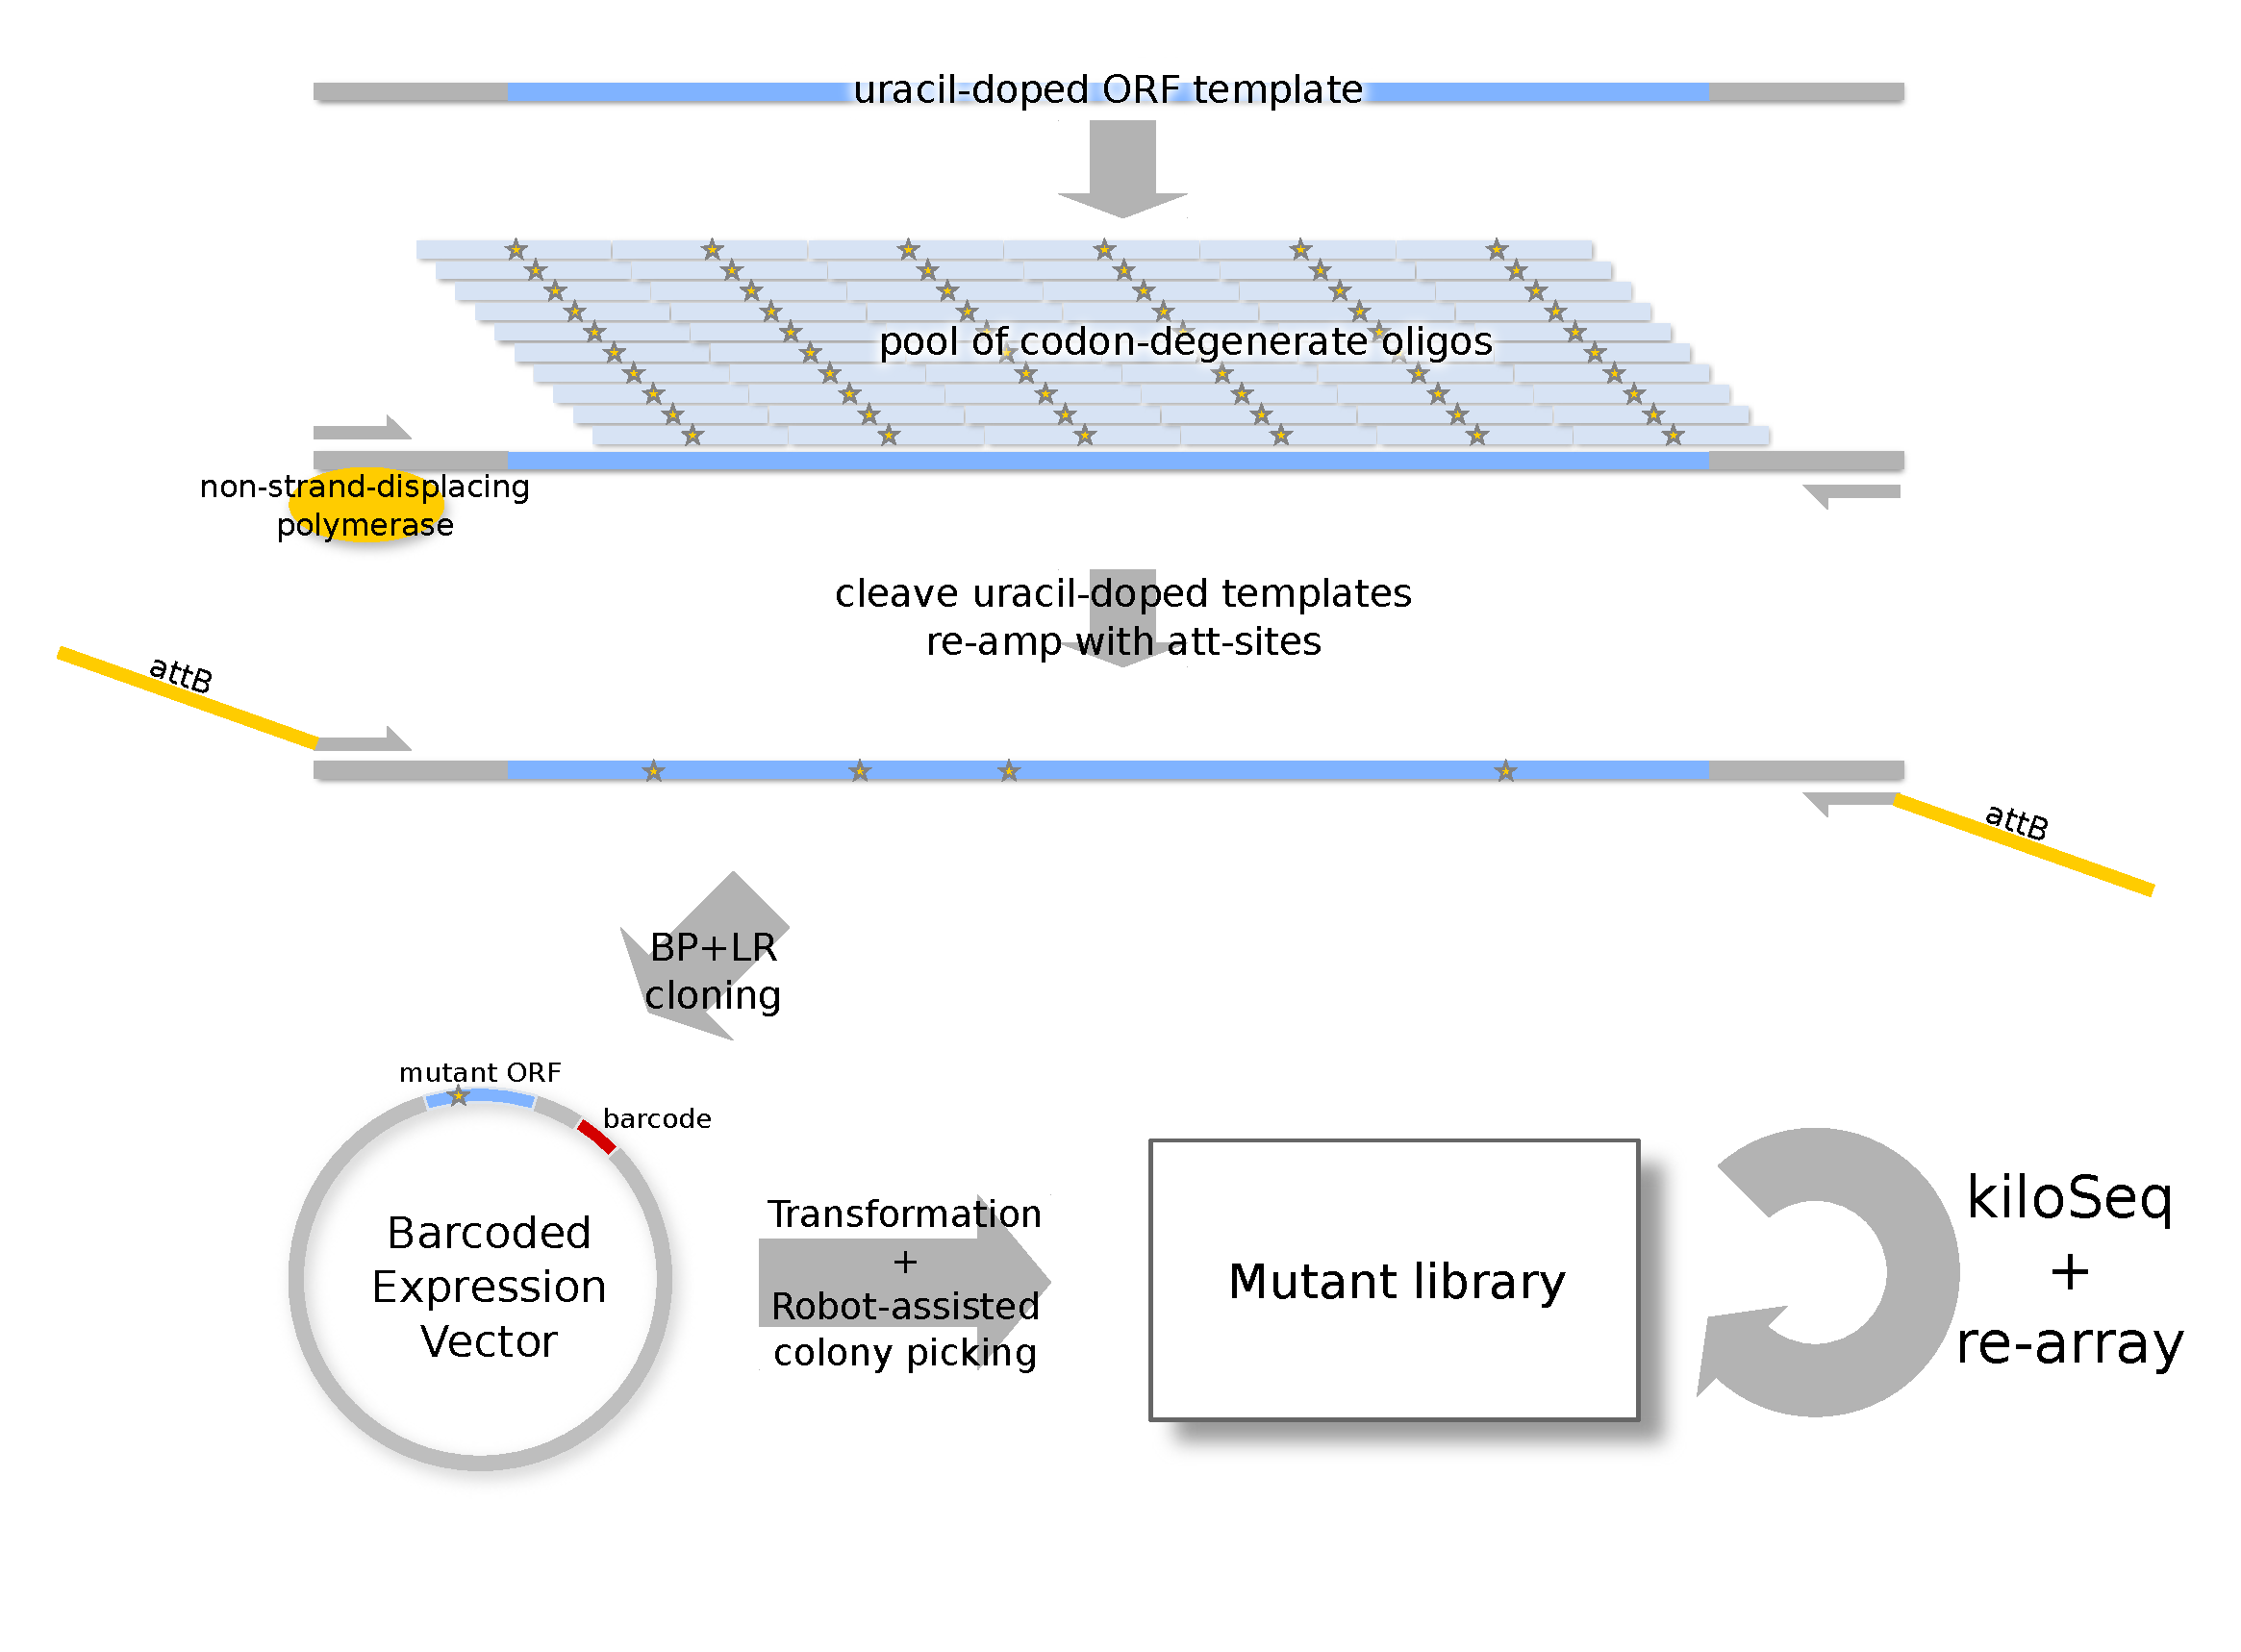
\includegraphics[width=\textwidth]{img/popcode_schema.pdf}
	\caption{POPCode mutagenesis and library generation. A pool of codon-denerate oligos is hybridized to a uracil-doped template, gaps between oligos are closed via non-strand-displacing polymerase, and the backbone sealed. Uracil-doped template is degraded to enrich for mutants. After mutagenesis, Gateway attB sites are added, followed by BP+LR cloning into barcoded vectors and transformation into bacteria. Finally, colonies are picked and arrayed. (Incl. illustration by~\cite{pire_stack_2012})}
	\label{fig:popcode_schema}
\end{figure}

Having designed and obtained suitable oligonucleotides, the ORF sequence is PCR amplified in the presence of dUTP to generate uracil-doped template for the mutagenesis reaction. Oligonucleotide pools are then hybridized with the template. Gaps between hybridizations are filled with non-strand-displacing polymerase. 
Following cleanup, the uracil-doped template is incapacitated using Uracil-DNA-Glycosylase (UDG). The mutagenesis product is then amplified with primers that add \texttt{attB} sites to allow for Gateway BP cloning into entry vectors.

To accomplish mutagenesis across the entire coding region of our gene of interest, \gene{UBE2I}, we designed a tiled collection of oligos using the web tool and applied POPCode to generate a codon-mutagenized amplicon library.  In parallel, we also carried out PCR with oxidized nucleotides~\cite{mohan_pcr_2011} to enable deeper representation of amino acid changes achievable from single-nucleotide changes.

\subsubsection{Library generation and highly multiplexed amplicon sequencing}

For Stage 2 of the framework---generation of a clone library---we employed an \textit{en masse} recombinational cloning strategy to generate a Gateway Entry vector library of \gene{UBE2I} variants. This library was transferred via \textit{en~masse} recombinational subcloning into a pool of randomly-barcoded plasmids enabling expression of \gene{UBE2I} variants in yeast. As sequencing is required to establish the full-length ORF sequence and barcode of each clone, the complementation vector is designed such that the variant ORF and the barcode locus are in close proximity to each other. Thus, only a relatively small segment of the plasmid needs to be inspected to determine the pairing of genotype and barcode. 

After bacterial transformation, we proceeded to robotically pick 19,968 colonies, which were stored in 52 384-well plates. As sequencing needs to be performed to catalogue the identities of nearly 20,000 individual samples, we used a novel sequencing method called KiloSeq which combines plate-position-specific index sequences with Illumina sequencing (Figure~\ref{fig:kiloseq_schema}).
KiloSeq was developed in collaboration with SeqWell Inc., Boston. First, for each clone in the library, the region of interest is amplified with primers containing well-specific tags, uniquely identifying each well coordinate. This step is dependent on the use of a HydroCycler, which allows up to 4608 PCR reactions to be performed in parallel. In the next step, wells for each plate can be pooled. Nextera tagmentation using Tn5 transposase is used to break the amplicons into random fragments and simultaneously ligate them to Illumina sequencing linkers with plate-specific indices. Then the pool is re-amplified with 3'-specific primers, to enrich for fragments that contain the well tags. The resulting library is now ready for paired-end sequencing. In each pair of reads, one read will contain the well tag and the barcode locus, whereas the other will contain a fragment of the mutant ORF.
%TODO: move to methods: This is done using a hydrocycler, allowing for thousands of PCR reactions to be performed in parallel. ----- Amplicons can then be plate-wise pooled.

\begin{figure}[h!]
	\centering
	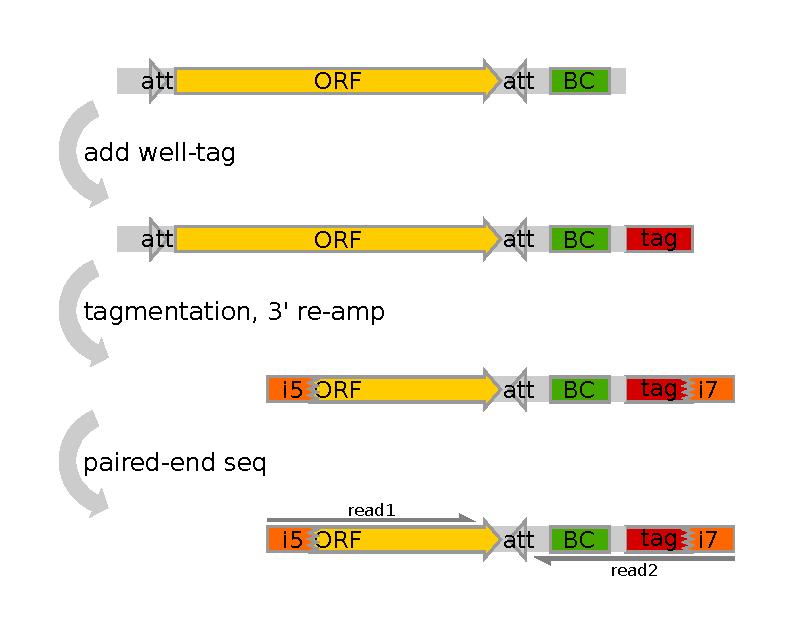
\includegraphics[width=.5\textwidth]{img/kiloseq_schema_new.pdf}
	\caption{KiloSeq schema. 1) For each library well, amplicons containing the variant ORF (gold) and Barcode locus (green) are amplified with primers adding a well-specific tag. 2) Tn5 tagmentation fragments the DNA while simultaneously adding Illumina i5/i7 linkers. 3' re-amplification enriches for fragments containing the well tags. 3) Each pair of sequencing reads now contains a fragment of ORF sequence and the associated barcode and well tag.}
	\label{fig:kiloseq_schema}
\end{figure}

To process the results of a KiloSeq sequencing run, I developed a custom-built software pipeline, which can be divided into three phases: demultiplexing; barcode clustering; and alignment and variant calling.
The first phase---demultiplexing---takes place on two levels, corresponding to library plates and the wells within those plates. Demultiplexing at plate level is performed by Illumina's \texttt{bcl2fastq} software, which resolves i5-i7 index combinations. The second phase is performed on a high performance computing cluster. Sets of read pairs are distributed across computing nodes, where they are processed by worker scripts. The well-tag within each R2 read is identified using a k-mer search algorithm, and read-pairs are sorted accordingly into bins. Each bin corresponds to one well in a given plate. At the same time, barcode sequences are extracted from the R2 reads in preparation for the next phase. 

The second phase---barcode clustering---uses the extracted barcode sequences within each bin and clusters them according to their Levenstein distance~\cite{levenshtein_binary_1966} (i.e. the number of edit operations required to transform one into the other). This step is necessary in order to resolve possible contamination across wells that occurred during library preparation. Each barcode cluster corresponds to a different clone, and the different unique sequences within each clusters correspond to different sequencing errors. The most frequently observed sequence within each cluster is interpreted as the true barcode. Finally, read pairs within each bin are again subdivided according to their respective barcode cluster.

The third phase---alignment and variant calling---is then executed for each barcode cluster within each well within each plate. The R1 reads are aligned to the template sequence and variants are called. This is complicated by the fact that the KiloSeq library preparation usually creates a certain amount of cross-contamination between wells. While single or multi-nucleotide variants are still relatively unproblematic to identify, standard tools were found to be unable to identify copy number variations (CNVs) due to these problems. I thus developed a custom method for CNV calling, based on detecting sudden changes in read depth across the alignments. First, the individual read depth track is normalized to the average read depth across all wells the plate. Then a modified one-dimensional Sobel operator~\cite{sobel_3x3_1968} is used to detect sharp edges in the signal. An example of this can be seen in Figure~\ref{fig:border_detect}. Detection thresholds were optimized by comparison with Sanger sequencing.

\begin{figure}[h!]
	\centering
	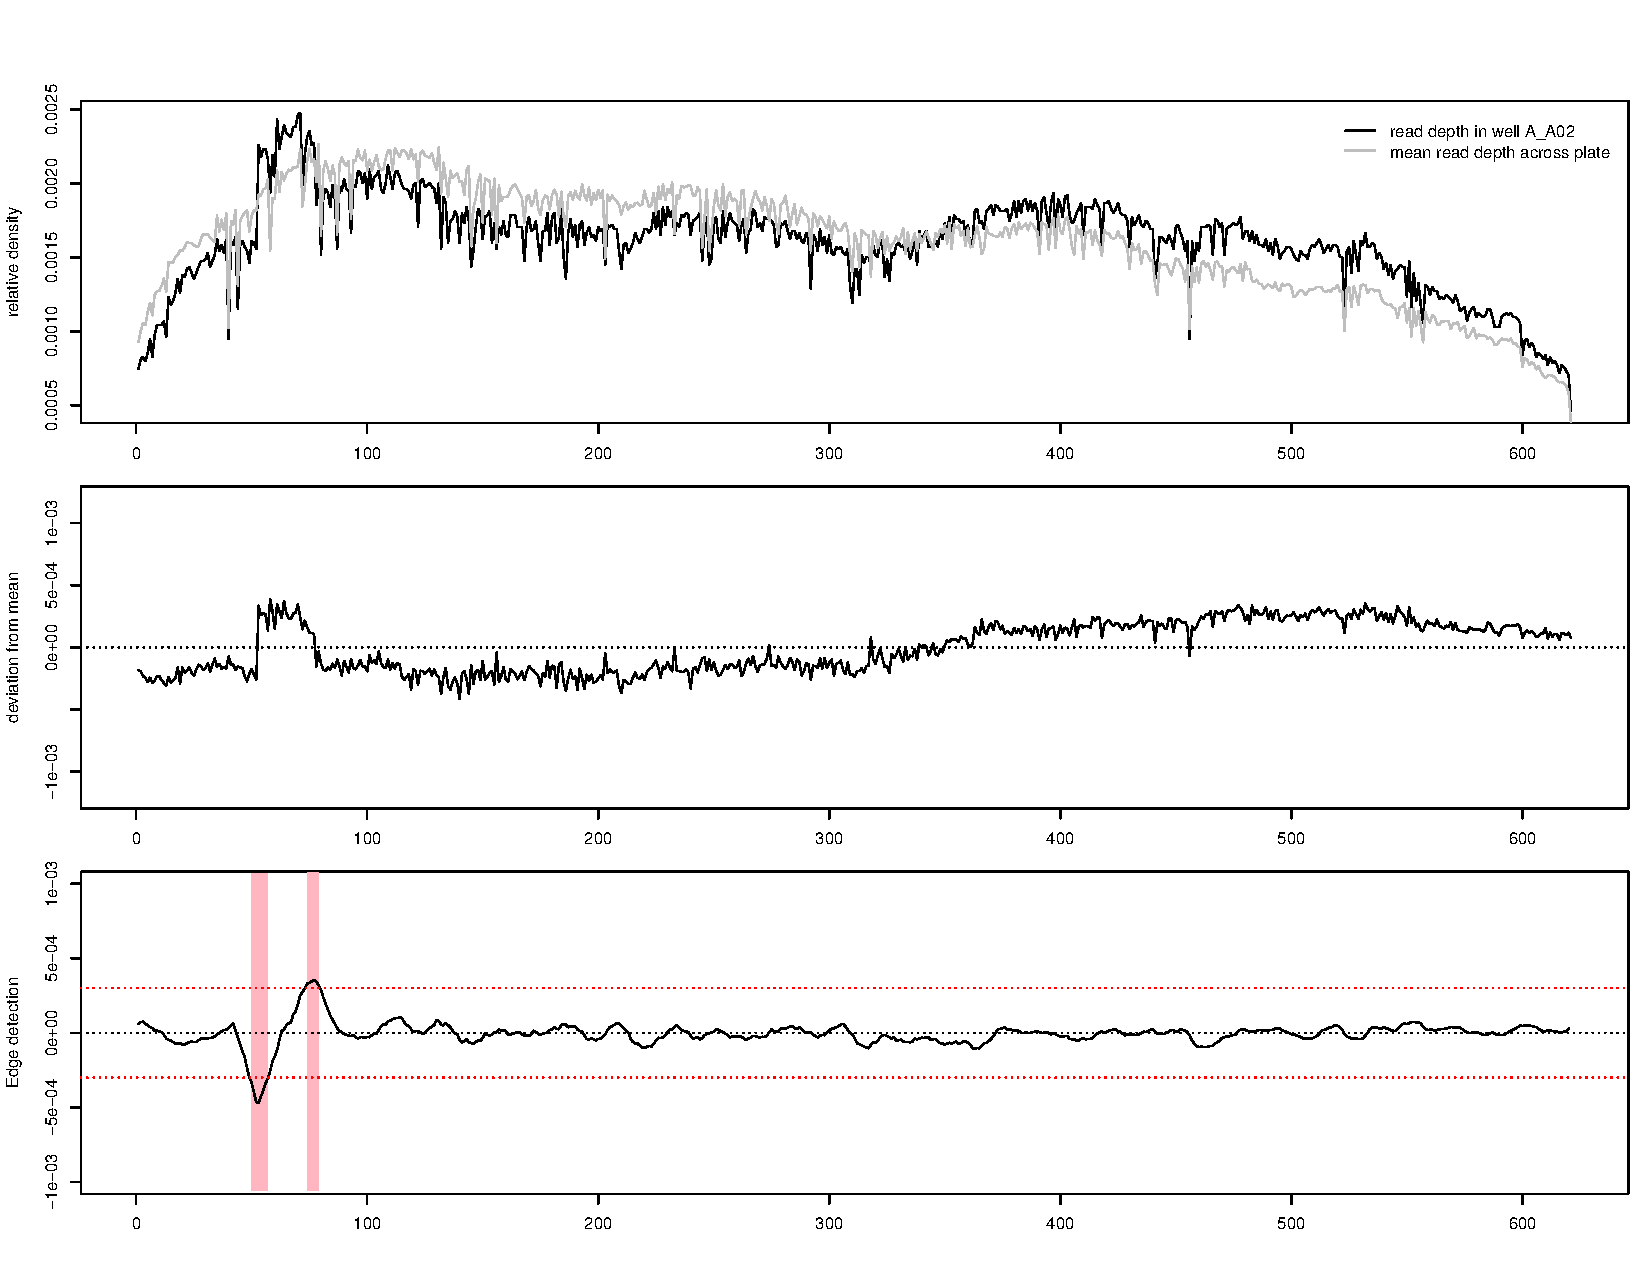
\includegraphics[width=\textwidth]{img/border_detect.pdf}
	\caption{Indel detection example. A duplication event in well \texttt{A\_A02} is detected by normalizing relative read depth by the mean depth across the plate and using a Sobel operator to detect sudden changes.}
	\label{fig:border_detect}
\end{figure}


After successful genotyping with kiloseq, I determined the subset of clones that (i) contained at least one missense mutation, (ii) did not contain any insertions or deletions, (iii) did not contain mutations outside of the ORF, (iii) had unique barcodes, and (iv) had sufficient read coverage during KiloSeq to allow for confident genotyping.
Over half of the clones in the library conformed to these criteria. The single largest reason for exclusion was the occurrence of indels and CNVs (Figure~\ref{fig:popcode_census}A). 

An analysis of the mutation signatures across clones generated by POPCode revealed that two different mechanisms appear to underlie mutagenesis. When considering only mutations that change more than one base in a given codon, there is an equal chance for every possible base except in the third position, where almost no adenine or cytosine was introduced. This is consistent with the \texttt{NNK} degeneracy code used in the POPCode oligo design. By contrast, variants that change only a single base in a given codon show a strong bias for transitions over transversions. These could be introduced due to polymerase error (Figure~\ref{fig:popcode_census}B). This secondary source of variation is also reflected in the relative share of single nucleotide variants, which make up 56\% of mutations (Figure~\ref{fig:popcode_census}C). As a consequence, when examining the mutation coverage across the sequence of the ORF, it is clearly visible that the share of amino acids reachable with a single nucleotide change from the respective wildtype codon is much closer to saturation than the the set of all possible amino acid changes (Figure~\ref{fig:popcode_census}D). Additionally, some hotspots are visible in which the mutation rate is higher, which is likely due to different hybridization efficiencies of oligos across the ORF sequence.

Using a pinning robot, we re-arrayed the subset of usable clones into a condensed final library of 40 plates. This final library comprised 6,553 \gene{UBE2I} variants, covering different combinations of 1,848 (61\% of all possible) unique amino acid changes. In preparation for the next stage, variant plasmids were pooled, together with barcoded empty vector and wild type control plasmids.

\begin{landscape}
\begin{figure}[h]
	\centering
	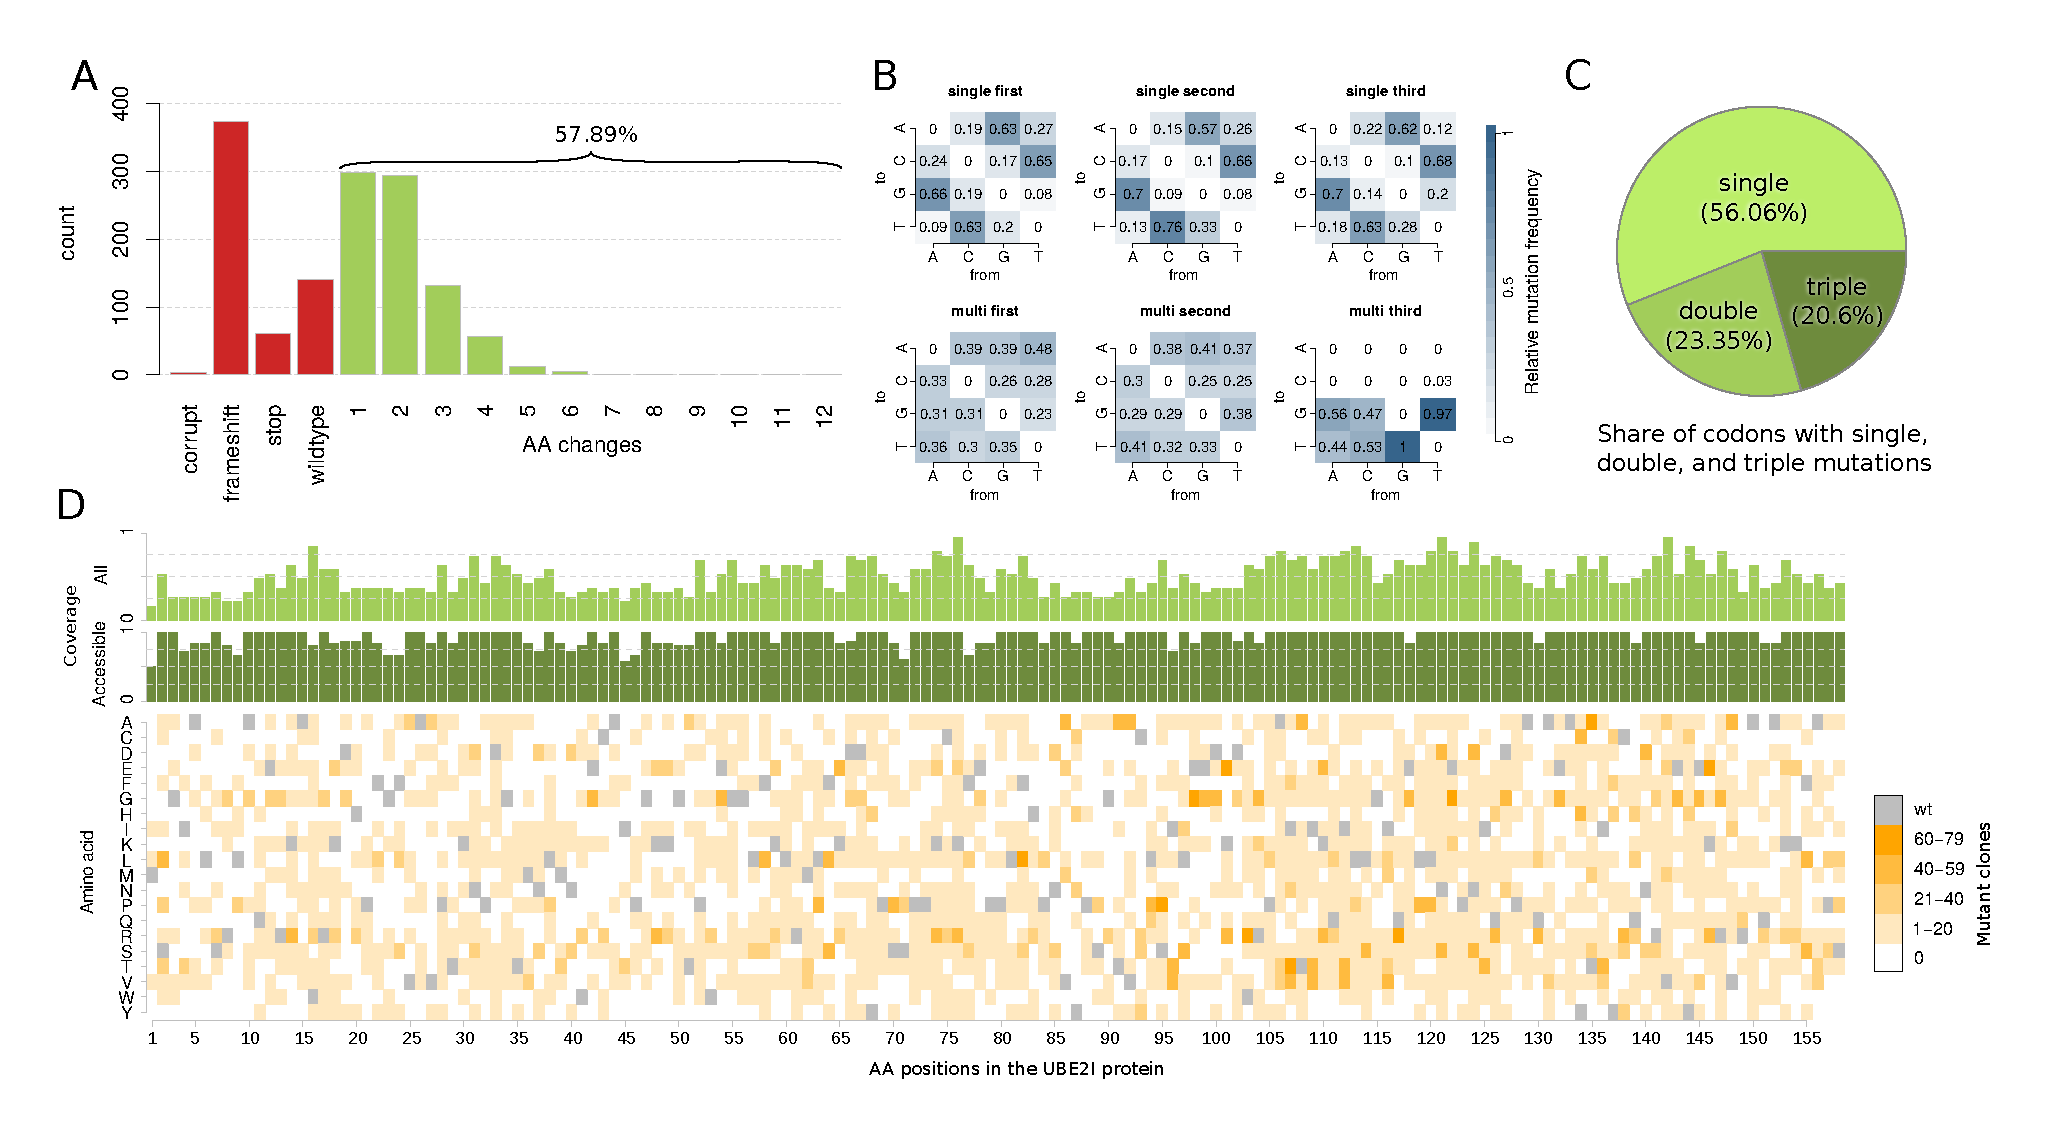
\includegraphics[width=9in]{img/popcode_census.pdf}
	\caption{KiloSeq-based census of the \gene{UBE2I} POPCode library. A) Breakdown of KiloSeq results for a set of five 384 well plates of mutant clones generated by POPCode. Corrupt: Clones containing mutations outside of the ORF; Frameshift: Clones containing indels or copy number variants; Stop: Clones containing stop codons. B) Breakdown of mutations in codons. Top: Single nucleotide variants; Bottom: Multi-nucleotide variants. Columns correspond to the first, second and third position in a codon. C) Relative shares of single, double and triple nucleotide variants among all missense variants in the library. D) Coverage map of missense variants in the library. Light green track: Coverage across all possible amino acids; Dark green track: Coverage across amino acids reachable with a single nucleotide change from the wildtype codon.}
	\label{fig:popcode_census}
\end{figure}
\end{landscape}



\subsubsection{Complementation screen and Barcode sequencing}

For Stage 3 of the DMS-BarSeq framework---the selection of clones encoding a functional protein---we employed a previously described \species{S.~cerevisiae} functional complementation assay~\cite{lee_complementation_1987,osborn_rescuing_2007}. This assay is based a yeast strain carrying a temperature sensitive (ts) allele of the \gene{UBE2I} orthologue \gene{UBC9}. Expression of human \gene{UBE2I} rescues growth at an otherwise lethal elevated temperature. As such, the fitness observed for a clone carrying a mutant allele of \gene{UBE2I} can be interpreted as the overall ability of the variant protein to function within its biological context~\cite{sun_extended_2016}. 
The plasmid library from Stage 3 was introduced into the appropriate ts strain by en-masse transformation. Pools were then grown in triplicates over a period of 48 hours at the permissive (25\celsius ) and selective (37\celsius ) temperatures, respectively (see Online Methods) and evaluated at multiple time points via high-throughput sequencing.

To facilitate the readout of the selection (Stage 4), I developed a sequence analysis pipeline. The pipeline distributes sets of read pairs across across the nodes of a high-performance computing cluster, where a k-mer search algorithm is used to identify multiplexing tags that encode the temperature and time point and replicate number associated with the sample. The same algorithm is also used to identify the barcode itself. The number of occurrences of each barcode in each sample is counted and aggregated across the cluster nodes. The frequencies at which each barcode is observed corresponds to the population size of the associated clone. This can then be used to reconstruct of individual growth curves and quantify the normalized fitness for each of the 6,553 strains (see Methods section for details). The fitness measurements are normalized to the wildtype and null controls, such that a score of 1 is equivalent to the average wildtype fitness, and 0 is equivalent to the average null control fitness.

Additional care needs to be taken to quantify the level of confidence for each fitness measurement. While comparing the three technical replicates available for each clone allows for a rough estimation of standard error, improvements can be made. Baldi and Long previously published a Bayesian method allowing for the regularization of variance estimations using prior data~\cite{baldi_bayesian_2001}. Two sources of prior information offer themselves: (1) The number of sequencing reads observed at time 0 of the experiment, as a low number indicates underrepresentation in the library, which is likely to result in a poor frequency estimate; and (2) the fitness estimate itself, as variance can be expected to be proportional to the mean. Indeed, when comparing both properties with the standard deviation, a clear trend is visible (Figure~\ref{fig:baldiLong}). After obtaining a prior estimate via linear regression, it can be used to regularize the empirical standard deviation.

\begin{figure}[h!]
	\centering
	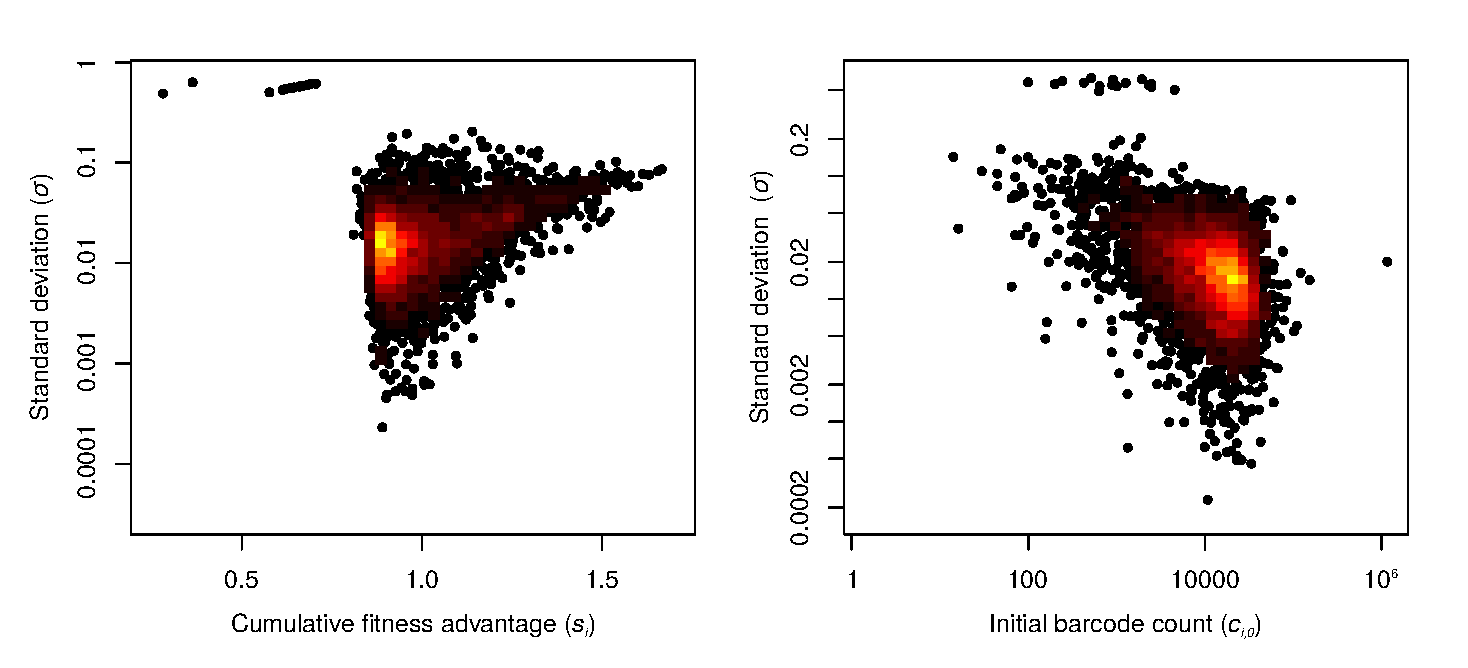
\includegraphics[width=\textwidth]{img/baldi_long.pdf}
	\caption{Comparison of fitness and initial barcode count against standard deviation. Both properties can be used as prior information to improve confidence quantification.}
	\label{fig:baldiLong}
\end{figure}


\subsubsection{A barcoded-based functional map of UBE2I}

Before further refinement in Stages 5 and 6, I assessed the quality of complementation scores. I first examined reproducibility of scores between technical replicates (Figure~\ref{fig:barseqValidation}A), and biological replicates (different clones carrying the same mutation; Figure~\ref{fig:barseqValidation}B).  In each case the scores were reproducible (Pearson's R of 0.97 and 0.78, respectively). We next carried out semi-quantitative manual complementation spotting assays for a subset of mutants that spanned the range of fitness scores. Complementation scores from deep mutational scanning correlated well with these small-scale tests. Indeed, agreement between the large-scale and manual scores was about the same as agreement between internal replicates of the large-scale scores (Figure~\ref{fig:barseqValidation}B,C). 

As a further sanity check, I next examined evolutionary conservation and common predictors of deleteriousness, such as PolyPhen-2~\cite{adzhubei_predicting_2001} and PROVEAN~\cite{choi_predicting_2012}.  Although each of these measures is far from perfect in predicting the functionality of amino acid changes, they should and did each correlate with functionality (Figure~\ref{fig:barseqValidation}D,E,F). Finally, I confirmed that, as expected, amino acid residues on the protein surface are more tolerant to mutation than those in the protein core or within interaction interfaces (Figure~\ref{fig:barseqValidation}G).  Taken together, these observations support the biological relevance of the DMS-BarSeq approach.

%TODO: Spacing issues in figure legend?

\begin{landscape}
\begin{figure}
	\centering
	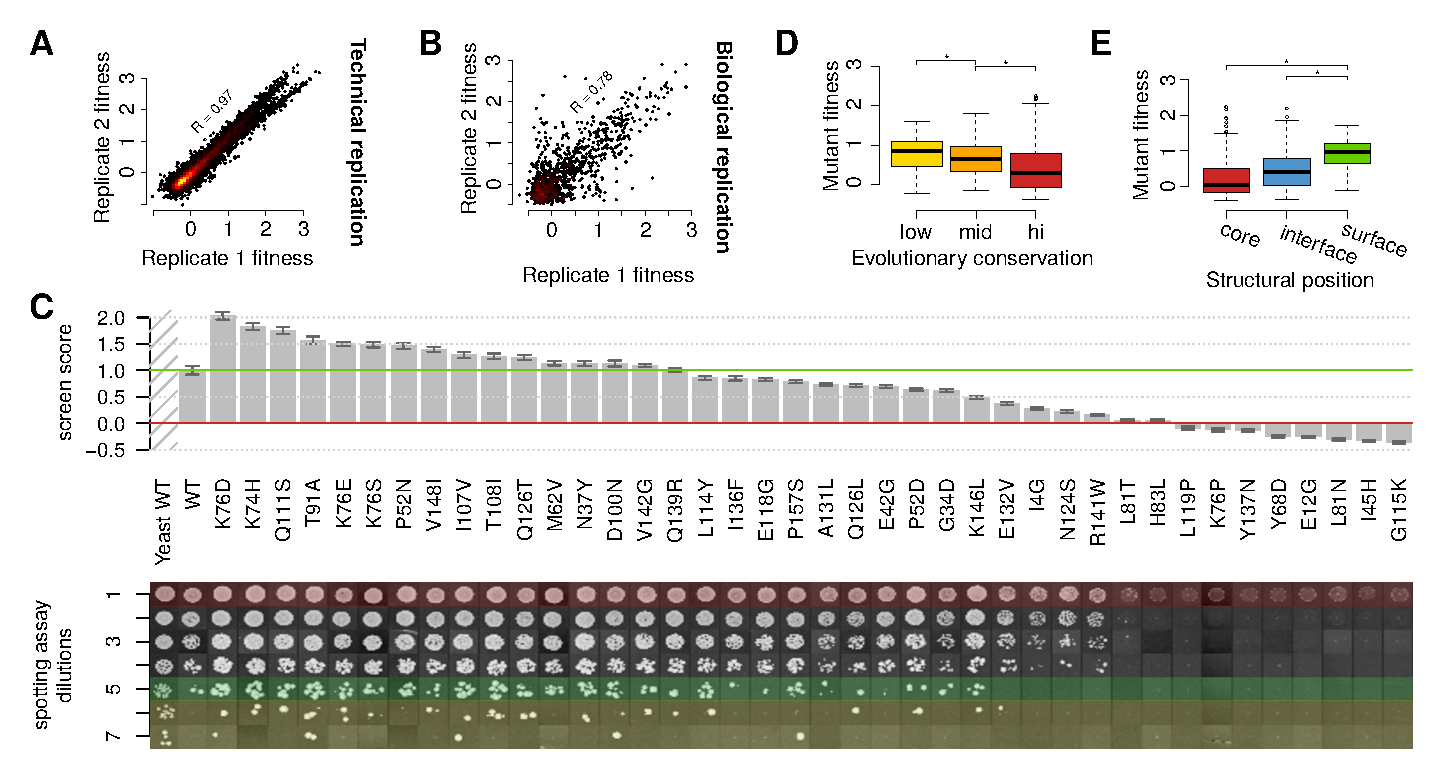
\includegraphics[width=9in]{img/barseq-validation.pdf}
	\caption{Validation of DMS-BarSeq of UBE2I. A: Correlation between technical replicates B: Correlation between biological replicates. C: Manual complementation spotting assay compared to DMS fitness measurements. D: Comparison of fitness levels for mutations at positions with low, medium and high evolutionary conservation. E: Comparison of fitness levels for mutations at positions within the hydrophobic core, at interaction interfaces, and unused surfaces}
	\label{fig:barseqValidation}
\end{figure}
\end{landscape}


\subsection{An alternative strategy for DMS via tiled regional sequencing}

While the DMS-BarSeq approach has many advantages (see Discussion), its performance comes at the cost of producing and maintaining an arrayed clone library, and of determining the full-length sequence of each coding region and barcode for each clone. We therefore investigated an alternative approach called DMS-TileSeq: Instead of tracking the fitness of each individual clone, we carried out \textit{en masse} measurements of the frequency of each variant in the pool before and after selection, by deep sequencing.  Sequencing was carried out for a set of short amplicon tiles that collectively encompass the complete coding region.  In this way, it is possible to discern the impact of each mutation by observing the impact of selection on the abundance of clones carrying this mutation.

In terms of mutagenesis (Stage 1), DMS-TileSeq is identical to DMS-BarSeq.  Given the mutagenized amplicon library, the cloning step (Stage 2) was carried out by \textit{en~masse} recombinational subcloning into complementation vectors (thus skipping the step of arraying and sequencing individual clones).  This plasmid pool was next transformed \textit{en~masse} into the \textit{ubc9-ts} strain appropriate for assessing the complementation ability of \gene{UBE2I} variants. As with DMS-BarSeq, DMS-TileSeq employs pooled strains grown competitively (Stage 3) at the permissive and selective temperatures. However, instead of using barcode sequencing to determine the fitness associated with individual stains, we directly sequence the coding region from the clone population to determine the frequency of each variant in each pool (before and after selection). To overcome the problem of distinguishing mutations from sequencing errors, we divide the coding region into tiles such that each individual template molecule can be completely sequenced on both strands.  By requiring that each variant be seen on both strands, the incidence of base-calling errors can be substantially reduced. %pipeline?

An important aspect of DMS-TileSeq is that it requires the library to be sufficiently complex to ensure that the effect of a mutation is determined from enough clones and averaged over enough genetic backgrounds to be reproducible. Therefore it was necessary to first validate the reliability of DMS-TileSeq in comparison to DMS-BarSeq on our established UBE2I map. Correlation between DMS-TileSeq and DMS-BarSeq was comparable to the correlation observed between biological replicates of DMS-BarSeq (Figure~\ref{fig:barVtile}A), suggesting that reproducibility of DMS-TileSeq is at least comparable to that of DMS-BarSeq. DMS-TileSeq and DMS-BarSeq showed similar agreement with complementation scores from manual assays (Figure~\ref{fig:barVtile}B). Thus, DMS-TileSeq avoids the substantial cost of arraying and sequencing thousands of individual clones, while performing on par with DMS-BarSeq in terms of reliability of the functional complementation scores it produces.

\begin{figure}[h!]
	\centering
	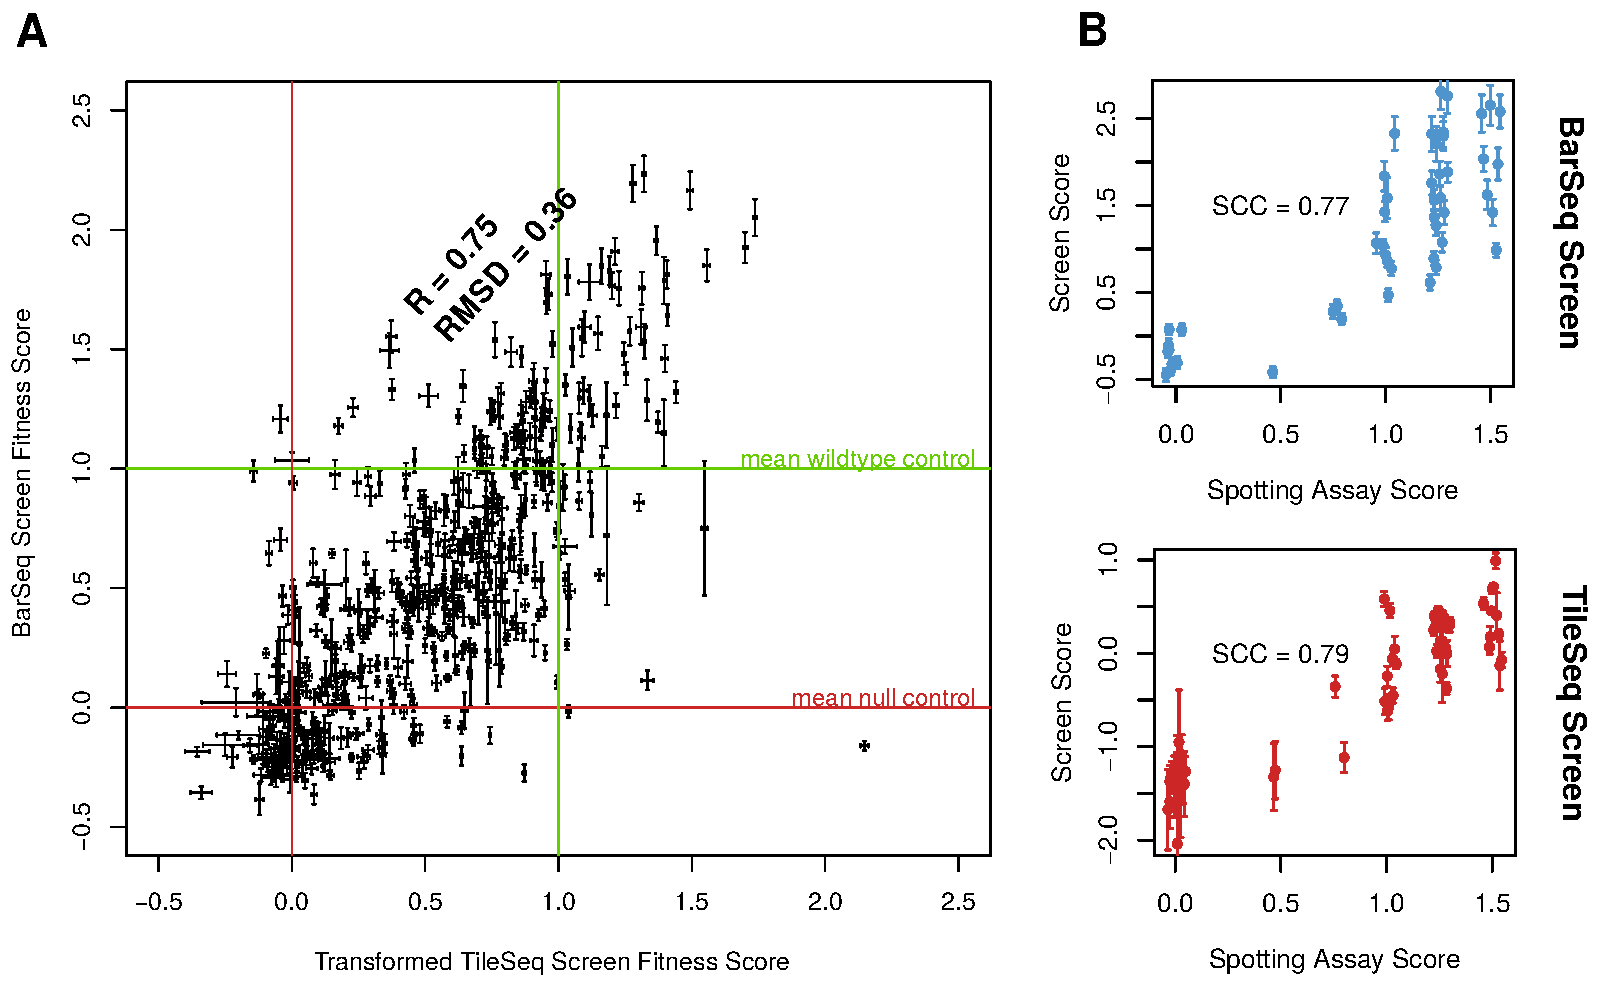
\includegraphics[width=.9\textwidth]{img/barVtile.pdf}
	\caption{Comparison of DMS-BarSeq to DMS-TileSeq scores. A) Scatterplot of functional scores for variants in obtained from BarSeq and TileSeq (transformed to the same scale), whisker bars show regularized standard error. B) Comparison of BarSeq (top) and TileSeq (bottom) scores to manual complementation spotting assay scores (jittered for visibility). Whisker bars show regularized standard error}
	\label{fig:barVtile}
\end{figure}

\subsection{A complete functional map of UBE2I}

Having performed two independent deep mutational scans of UBE2I using functional complementation assays, we wished to integrate both results into a single comprehensive high-quality map. To accomplish this, I first combined the results of each screening approach into a joint map.  This required bringing the maps onto the same scale. Using a regression-based transformation function, I transformed the DMS-TileSeq scores to the more intuitive scale of DMS-BarSeq (where 0 corresponds to the typical score of a null mutant and 1 corresponds to the typical score of a wildtype control). I then combined scores from the two methods, giving greater weight to more confident measurements (see methods section).

\subsubsection{Imputation and regularization of missing or less accurate data}

As is the case for all previously published DMS maps, our combined map contained some entries that were poorly measured or missing (e.g., because these substitutions were underrepresented in the input clone library). To fill the gaps in the map (Stage 5 in the framework), I trained a Random~Forest~\cite{breiman_random_2001} regression model using the existing measurements in the map. The features used for the model fall into four categories: intrinsic information; conservation information; chemicophysical properties; and structural properties. 

The most important intrinsic feature consists of weighted positional averages in the map. That is, for any given amino acid change, all other observed effects of variants at the same amino acid position are weighted according to their measurement confidence and are then used to form an average. A second intrinsic feature consists of the confidence-weighted average effect of all variants containing the amino acid change in question. Finally, as a third intrinsic feature I calculate the expected variant fitness predicted by a multiplicative model often applied to detect genetic interactions~\cite{phillips_language_1998,onge_systematic_2007}. In the absence of interaction, the fitness of a double mutant $f_{A,B}$ is expected to follow the product of the individual single mutant fitness levels $f_{A,B}\approx f_A \cdot f_B$. Thus, in cases where a double mutant $(A,B)$ and a single mutant $B$ is known, the fitness of $A$ can be estimated to be $f_A\approx \frac{f_{A,B}}{f_B}$. The model is applied to all available double mutant fitness values carrying the mutation in question in combination with available complementary single mutant fitness values. As the latter two features rely on multi-mutant fitness measurements, they can only be applied where DMS-BarSeq data is available. 

The second category of features focuses on evolutionary conservation. For each amino acid change in question, this encompasses the corresponding BLOSUM62~\cite{henikoff_amino_1992}, SIFT~\cite{ng_predicting_2001} and PROVEAN~\cite{choi_predicting_2012} scores, and the AMAS~\cite{livingstone_protein_1993} conservation at the given position. The third category of features comprises chemicophysical properties such as mass and hydrophobicity of the original and wildtype amino acids and the difference between the two. The fourth and final category of features consists of structural properties of the affected amino acid residues, such as solvent accessibility, engagement in polar interactions and burial in interaction interfaces.

\begin{landscape}
\begin{figure}[h]
	\centering
	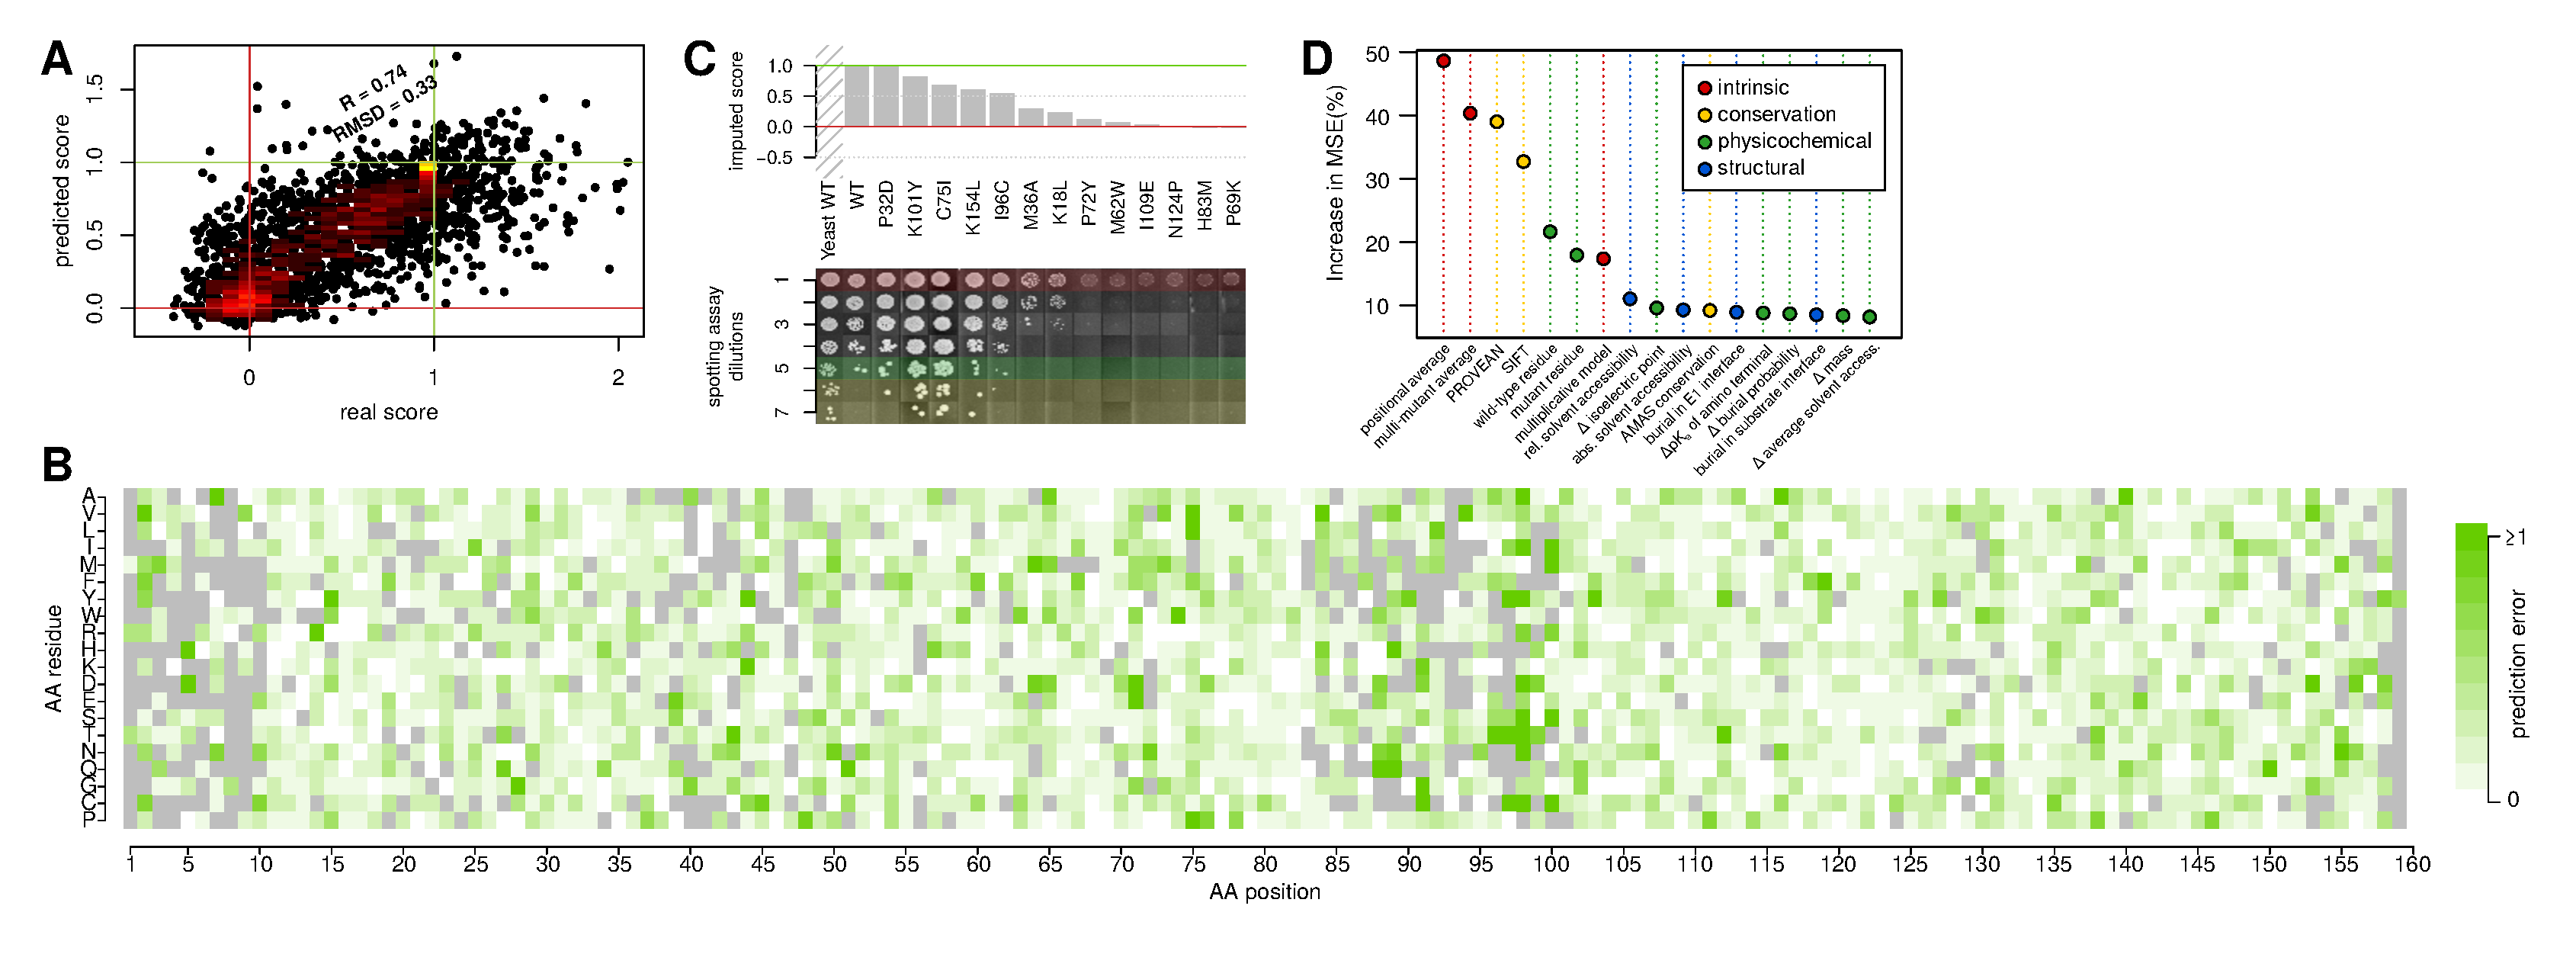
\includegraphics[width=9in]{img/imputation.pdf}
	\caption{Evaluation of machine learning imputation. A) Cross-validation correlation between measured values and machine learning predictions. B) Cross validation prediction error landscape. C) Manual complementation spotting assay compared to machine learning predictions for an independent test set of variants not present in the training data. D) Feature importance as measured by average increase in mean squared error.}
	\label{fig:imputation}
\end{figure}
\end{landscape}

I assessed the performance of the imputation model using cross-validation. Surprisingly, I found the root-mean-squared deviation (RMSD) of imputed values to be on par with measurement error in experimentally measured data (Figure~\ref{fig:imputation}A). An examination of the prediction performance by location showed increased error in positions with lower mutation density and for variants with above-WT fitness levels (Figure~\ref{fig:imputation}B). As an additional validation step, we performed manual complementation assays for a set of UBE2I variants that were not present in the machine learning training data set and compared the results against the predictions (Figure~\ref{fig:imputation}C), again finding a surprisingly strong agreement. Notably, variants showing above wild-type level growth in the manual assay were generally predicted to be deleterious. Although above-WT complementation may indicate that a variant is adaptive in yeast, the imputation models suggested that these variants would be deleterious in humans, a hypothesis that is explored further in chapter~\ref{ch:data2}. 


An analysis of feature importance can be performed by comparing the increase in the mean squared prediction error upon permuting the values of a feature in question. The analysis revealed that intrinsic features were the most informative (Figure~\ref{fig:imputation}D), with the weighed position-wise average and multi-mutant average seen to be the two single most important features (49\% and 40\%, respectively), while the multiplicative model contributed 14\%. The second most important group was conservation information, with PROVEAN and SIFT weighing in at 39\% and 32\%, respectively.

\begin{figure}[h!]
	\centering
	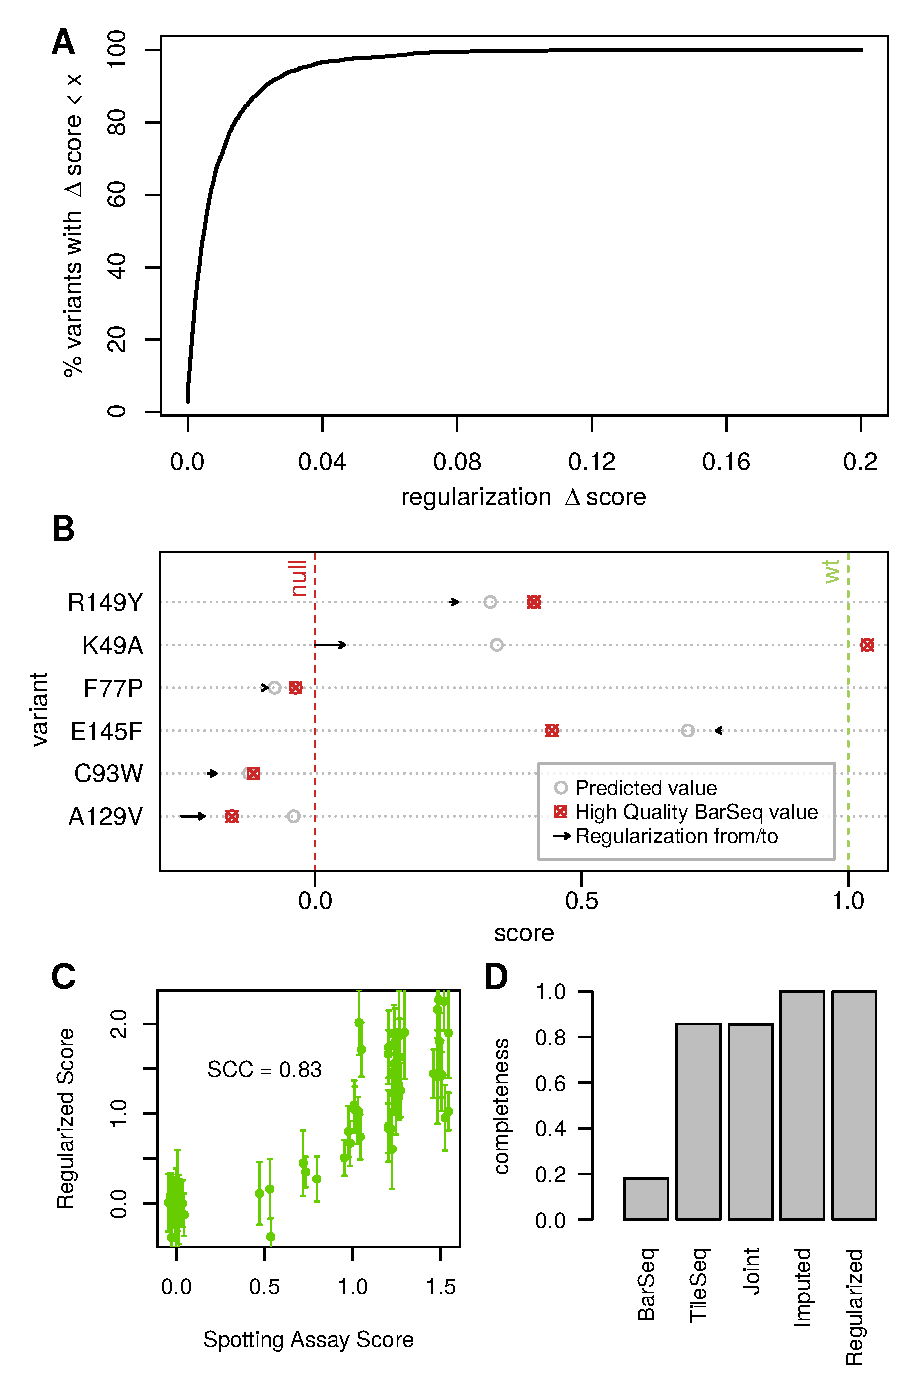
\includegraphics[width=.7\textwidth]{img/regularization_eval_ube2i.pdf}
	\caption{A) Cumulative distribution of changes to the fitness scores on the map as a result of regularization. B) Six variants were that were well measured in DMS-BarSeq but less well measured in DMS-TileSeq. For evaluation, regularization was performed only on the DMS-TileSeq data and compared to the DMS-BarSeq gold standard. Base and tip of arrows indicate pre- and post-regularization values, gray circles indicate the machine learning predictions used. Red targets indicate BarSeq gold standard. C) Comparison of values in the regularized map against manual complementation spotting assay values. D) Completeness of the map (in terms of coverage of possible amino acid changes) at different stages of the framework.}
	\label{fig:regularization}
\end{figure}

Finally, in stage 6 of the DMS framework, we wished to address cases in which experimental measurements were available but less confident. I implemented a regularization method, combining experimental measurements with machine-learning predicted values after dynamically weighting them according to their respective confidence levels. That means: the less confident a measurement, the stronger the regularization. Overall, most values were only adjusted minimally through regularization, with 90\% of values being altered by less than 2.5\% of the score difference between null and wt controls (Figure~\ref{fig:regularization}). This reflects the fact that most values were already of high quality. 

To evaluate the effect on the minority of variants that required stronger regularization, I looked for cases that were of low quality in the DMS-TileSEQ dataset, but well measured in the DMS-BarSeq experiment. This would allow me to treat the DMS-BarSeq values as a gold-standard basis of comparison when performing the regularization procedure only on the DMS-TileSeq dataset. I identified six cases that fulfilled these criteria. In all six cases regularization of DMS-TileSeq resulted in improvement, i.e. adjusted the corresponding values such that they more closely resembled the gold standard (Figure~\ref{fig:regularization}B). However, I found the changes to be still very conservative. More drastic weighting towards the machine learning prediction could have improved these cases even more.

To evaluate the complete map, we once more applied manual complementation assays to a set of variants that represented the full range of fitness scores.  DMS fitness scores corresponded closely with manual assays (Figure~\ref{fig:regularization})C, with a Spearman correlation of 0.83 between the high-throughput and low-throughput values (a slight improvement of 0.06 compared to the raw, unregularized experimental data).


\section{Discussion}

Here I have demonstrated the capabilities of a new improved Deep Mutational Scanning framework that uses functional complementation in yeast to map the impact of mutations on the overall ability of a protein to function. I integrated a machine learning-based imputation and regularization strategy into the deep mutational scanning process, to create the first DMS map that is complete with respect to high-quality functional impact scores over the full length of a protein. 

The two versions of DMS described, DMS-BarSeq and DMS-TileSeq, each have advantages and limitations. DMS-BarSeq permits study of the combined effects of mutations located at any distance along the clone, and therefore can reveal intramolecular genetic interactions (as will be explored further in the next chapter).  Futhermore, mutant clones produced for DMS-BarSeq are arrayed, sequenced and indexed which enables potential follow up investigation of individual variants. DMS-BarSeq also allows for the direct comparison of growth of any clone to null and wild type controls, resulting in an intuitive scoring scheme. However, the cost of arraying and sequencing clones for DMS-BarSeq renders it more costly and labour intensive, even given the efficient KiloSeq strategy. By contrast, the regional sequencing strategy of DMS-TileSeq is substantially more efficient, but can only analyze fitness of those double mutant combinations that fall within the same tile. 

The use of codon-replacement mutagenesis allows for the observation of a fuller repertoire of amino-acid substitutions than single-nucleotide mutagenesis would have allowed (only $\sim~30\%$ of all possible amino acid substitutions are accessible by single nucleotide mutation).  However, given that the majority of missense variants observed in individual genomes are single-nucleotide variants~\cite{lek_analysis_2016}, one might reasonably wonder whether codon mutagenesis is worth carrying out in addition to single-nucleotide mutagenesis.  There are three arguments for using codon-level mutagenesis to reveal the impact of all 19 possible amino acid substitutions at each position:  1) a full picture of functional missense variation enables a clearer understanding of what biochemical properties are required of each functionally important residue; 2) an analysis of over 60,000 unphased human exomes~\cite{lek_analysis_2016} found that each individual human harbors approximately 23 codons containing multiple nucleotide variants that collectively encode an amino acid not encoded by either single variant; 3) it seems likely that, going forward, the dominant cost of DMS will be development and validation of the functional assay, so that carrying out codon-level mutagenesis instead of (or in addition to) nucleotide-level mutagenesis has a relatively small impact on overall cost.


\section{Methods}

\subsection{Mutagenesis and library construction}

\paragraph{Oxidized nucleotide PCR: } Oxidized nucleotide PCR was performed by Jennifer Knapp as previously described by Mohan and colleagues~\cite{mohan_pcr_2011}. A 100$\upmu$M dNTP mixture was incubated at 37\celsius\ with 5mM $\text{FeSO}_4$ for 10 minutes. Addition of 0.5M Mannitol was used to stop the reaction. Oxidized nucleotides were prepared fresh for every PCR reaction.
PCR in presence of oxidized nucleotides. PCR reaction containing: 1-5ng template DNA, $1\times$ Thermopol Buffer (Invitrogen), 1.5mM $\text{MgCl}_2$, 0.2mM dNTP, 0.33$\upmu$M forward and reverse primers containing attB sites, 1U Taq polymerase was set up during the nucleotide oxidation reaction. Oxidized nucleotides were the last component added to the PCR reaction at a concentration of 0.1mM (half the amount of regular dNTP). Thermal cycler program: 95\celsius\ for 10 min, 30 cycles of 95\celsius\ for 1 min, 50\celsius\ for 1 min, 72\celsius\ for 1 min, final extension at 72\celsius\ for 10 min. Mutagenized PCR product was visualised on a 1\% agarose gel, and gel-extracted using a gel extraction kit (Qiagen). The gel extracted PCR product is the pooled mutagenesis product carrying \textit{attB} sites that is carried through to the KiloSeq stage.

\subsubsection{POPCode mutagenesis} 
\paragraph{Oligonucleotide design:} POPCode oligos are generated using the POPCodeSuite webtool I created. Given a target oligo length and a maximum length offset, the tool calculates for every codon in the target gene the set of possible oligos conforming to the length and offset parameters. Then, melting temperatures for the 5' and 3' halves of each oligo are calculated. For each codon, the oligo that most closely matches the median 5' and 3' melting temperatures is chosen. Based on parameters derived from previous observations, the expected mutation frequency is calculated for each oligo and used to simulate variant coverage rates at different library sizes. The source code is provided on the attached storage media and can also be found online\footnote{
\url{http://dalai.mshri.on.ca/~jweile/projects/popcodeSuite/}
}.

The POPCode mutagenesis protocol was performed by Atina Cot\'e, Jennifer Knapp and Marta Verby in the following steps: (i) the uracil-containing wild type template was generated by PCR-amplifying the ORF with dNTP/dUTP mix and HotTaq DNA polymerase, (ii) the mixture of phosphorylated oligonucleotide pool and uracil-containing template was denatured by heating it to 95\celsius\ for 3 minutes and then cooled down to 4\celsius\ to allow the oligos hybridize to the template, (iii) gaps between hybridized oligonucleotides were filled with the non-strand-displacing Sulpholobus Polymerase IV (NEB) and sealed with T4 DNA ligase (NEB), (iv) after degradation of the uracil-doped wild-type strand using Uracil-DNA-Glycosylase (UDG) (NEB), the mutant strand was amplified with attB-sites-containing primers and subsequently transferred en masse to a donor vector by Gateway BP reaction to generate a library of entry clones. 

\paragraph{Synthesis of uracil-containing template:} A 50$\upmu$l PCR reaction contained the following: 1ng template DNA, $1\times$ Taq buffer, 0.2mM dNTPs-dTTP, 0.2mM dUTP, 0.4$\upmu$M forward and reverse oligos, and 1U Hot Taq Polymerase.  Thermal cycler conditions are as follows: 98\celsius\ for 30s, 25 cycles of 98\celsius\ for 15s, 60\celsius\ for 30s, and 72\celsius\ for 1min. A final extension was performed at 72\celsius\ for 5 min.  Uracilated amplicon was gel-purified using the Minelute gel purification kit (Qiagen). 

\paragraph{Phosphorylation of mutagenic oligos:}  Desalted oligos were purchased from Eurofins and Thermo Scientific. The phosphorylation reaction is as follows: a 50$\upmu$l reaction containing $1\times$ PNK buffer, 300 pmol oligos, 1mM ATP, and 10U Polynucleotide Kinase (NEB) was incubated at 37\celsius\ for 2 hours.  The reaction was used directly in the subsequent POPCode reaction. 

\paragraph{POPCode oligo annealing and fill-in:} A 20$\upmu$l reaction containing 20ng uracilated DNA, 0.15$\upmu$M phosphorylated oligo pool, and 1.5$\upmu$M 5'-oligo was incubated at 95\celsius\ for 3 minutes followed by immediate cooling to 4\celsius.  A 30$\upmu$l reaction containing $1\times$ Taq DNA Ligase buffer, 0.2mM dNTPs, 2U Sulfolobus DNA Polymerase IV (NEB), and 40U Taq DNA Ligase (NEB) was added to the DNA and was incubated at 37\celsius\ for 2 hours. 

\paragraph{Degradation of wild-type template:} 1$\upmu$l fill-in reaction was added to a 20$\upmu$l reaction containing $1\times$ UDG buffer and 5U Uracil DNA Glycosylase (NEB) and incubated at 37\celsius\ for 2 hours.

\paragraph{Amplification of mutagenized DNA:} 1$\upmu$l UDG reaction was added to a 50$\upmu$l reaction containing $1\times$ Taq buffer, 0.2mM dNTPs, 0.4$\upmu$M forward and reverse oligos, and 1U Hot Taq Polymerase.  Thermal cycler conditions are as follows: 98\celsius\ for 30s, 25 cycles of 98\celsius\ for 15s, 60\celsius\ for 30s, and 72\celsius\ for 1min. A final extension was performed at 72\celsius\ for 5 min.

\subsubsection{Library construction}
Library construction was performed by Atina Cot\'e, Jennifer Knapp and Marta Verby following the \textit{en masse} LR cloning protocol previously described in Yachie \etal\ \cite{yachie_pooledmatrix_2016}. 

\paragraph{Generation of mutagenised pool of Entries:} An \textit{en masse} Gateway BP reaction containing 150ng of pooled mutagenesis PCR product carrying \textit{attB} sites, 150ng of pDONR223, 1$\upmu$L Gateway BP Clonase II Enzyme Mix (Invitrogen), $1\times$ TE Buffer is prepared. This reaction is incubated overnight at room temperature and then transformed into \species{E.~coli} aiming for the maximum number of transformants (at least 100,000 CFUs) to keep complexity high. Several colonies are picked at this stage for a quality control check by Sanger sequencing, and the rest are put through a pooled DNA extraction. The result is a pool of mutagenised PCR product inserted into the entry vector pDONR223.

\paragraph{Generation of Barcoded Destination Pools:} Barcoded destination plasmids were generated as previously described in Yachie~\etal\ \cite{yachie_pooledmatrix_2016}, but instead of being arrayed were maintained as pools with high complexity. Briefly, a linear PCR product containing two random 25 nucleotide barcode regions along with common linker sequences for priming was combined with a Gateway-compatible vector at a SacI restriction site through \textit{in vitro} DNA assembly~\cite{gibson_enzymatic_2009}. This barcoded destination vector pool was transformed into One Shot ccdB Survival T1R Competent Cells (Invitrogen). The transformations were spread onto large round LB+ampicillin petri plates for increased selection capacity and pool complexity was estimated from CFU counts. The plates were combined into a single pool for plasmid DNA extraction by maxiprep.

\paragraph{En masse Gateway LR reaction:} An \textit{en masse} Gateway LR reaction was used to transfer the mutagenised pool of entries into the barcoded destination pool. This reaction takes place over five days. On Day 1, a 5$\upmu$L reaction containing 150ng of mutagenised ORF pool in pDONR223 backbone, 150ng barcoded pHYC expression vector pool, 1$\upmu$L LR Clonase II Enzyme Mix, $1\times$ TE buffer is prepared. The reaction is incubated at room temperature overnight. On each of days 2-5, add in a 5$\upmu$L volume consisting of 150ng barcoded pHYC expression vector, 1$\upmu$L LR Clonase II Enzyme Mix, $1\times$ TE Buffer, incubating at room temperature overnight each day. On day 5, the final volume is 25$\upmu$L. 

\paragraph{Transformations and colony picking:} LR reactions were transformed into \species{E.~coli} and plated to achieve a density of 400-600 individual colonies per plate. A Biomatrix robot (Biomatrix BM5-BC robot, S\&P Robotics) was then used to automatically pick and array 384 colonies per plate for a total of $\sim$20,000 clones in $\sim$52 plates per ORF of interest. Each colony at this stage should contain a pHYC expression vector harbouring a variant of the ORF of interest and a unique barcode.

\subsection{KiloSeq and library condensation}

\paragraph{Experimental procedures:} KiloSeq library preparation was performed by Atina Cot\'e, Jennifer Knapp and Marta Verby. 
%384-well plates are prepared with PCR mastermix, where each well contains differently tagged oligos representative its respective well coordinate. A Biomatrix BM5-BC robot (S\&P Robotics) is used to stamp clones directly from the library plates into the wells. Colony PCR is performed directly in the plates using a Hydrocycler 16 (LGC Group, Ltd.). Wells across each plate are then pooled and fragmented using Nextera Tn5 tagmentation. Fragments carrying the well-specific tags within each pool are then re-amplified using primers carrying Illumina i5/i7 linkers with plate-specific indices. Finally, the products are pooled, purified and size selected.
The first step is to PCR-amplify a segment of the plasmid containing both ORF and barcode locus. PCRs were carried out using the Hydrocycler 16 (LGC Group, Ltd.), using primers with well-specific index sequences. Amplicons from each plate were pooled, and subjected to Nextera ‘tagmentation’ using Tn5 transposase to generate a library of amplicons with random breaks to which the adapters have been ligated. The fragments are then re-amplified to generate a library of amplicons such that one end of each amplicon bears the well-specific tag and the other (ladder) end bears the Nextera adapter. These libraries can be re-amplified to introduce Illumina TruSeq adaptors, allowing multiple plates of amplicons to be sequenced together.  Paired-end sequencing was carried out using Illumina NextSEQ 500. In each pair of reads, one read will reveal the well tag and the barcode locus, whereas the other will contain a fragment of the mutant ORF, and these fragments can be assembled into a contiguous sequence.


\begin{figure}[h!]
	\centering
	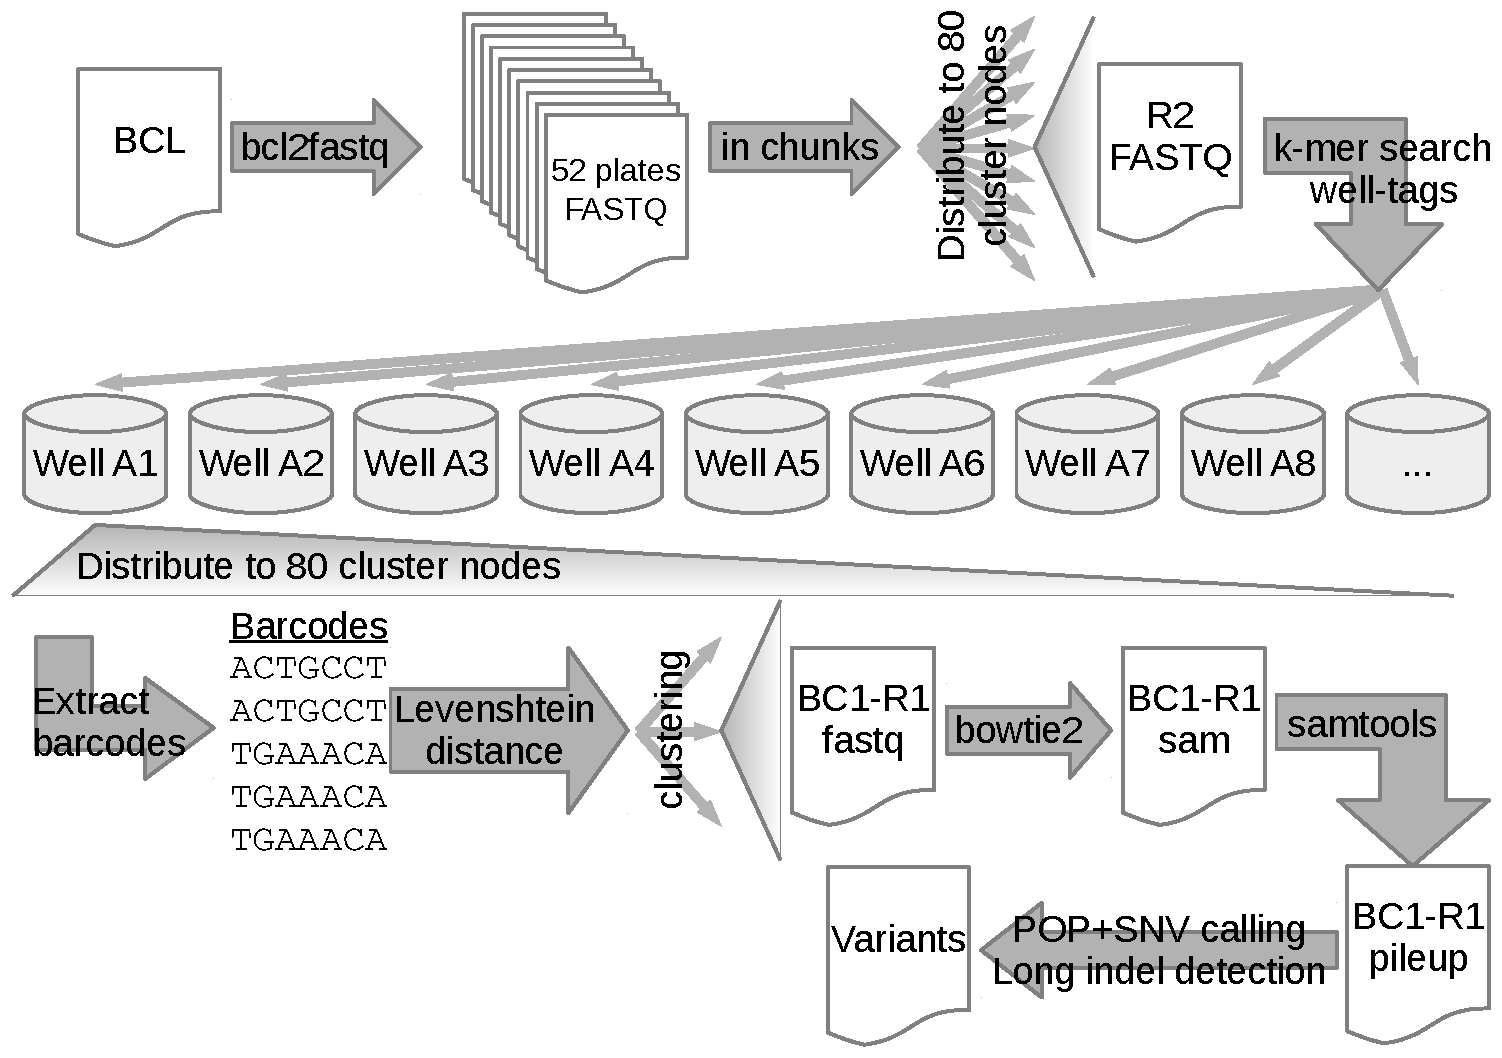
\includegraphics[width=.6\textwidth]{img/kiloseq_pipeline.pdf}
	\caption{KiloSeq analysis pipeline: \texttt{bcl2fastq} is used to demultiplex by plate. The resulting FASTQ files are broken up in to chunks and feed to worker nodes on the fly. Each worker identifies well-tags in the R2 reads and demultiplexes by well accordingly. After demultiplexing is complete, jobs for each well in each plate are distributed across worker nodes. There, barcode sequences are extracted and clustered based on Levenshein distance. R1 reads from each cluster are aligned to the ORF reference and pileups are generated, which are used for variant calling and long indel detection (via recognition of sudden changes in read depth using a modified Sobel filter.)}
	\label{fig:kiloseqPipeline}
\end{figure}


\paragraph{Computational procedures:} I developed a sequence analysis pipeline to process all KiloSeq data. The pipeline runs on a high-performance computing cluster (Figure~\ref{fig:kiloseqPipeline}).
In the first step, Illumina \texttt{bcl2fastq} is used to demultiplex the reads at the plate level using the custom Nextera indices. The resulting \texttt{FASTQ} files are then further demultiplexed using the well-tags in a highly parallel fashion. This results in a folder structure containing tens of thousands of individual \texttt{FASTQ} files sorted by plate and well location. These are then further processed in parallel to identify barcodes. Wells can sometimes contain more than one clone (e.g., due to incomplete washing in the robotic pinning process). Thus barcode sequences are extracted from each read and then clustered by edit distance~\cite{levenshtein_binary_1966} to determine the set of barcodes in each well. The associated paired reads for each barcodes are then further split by barcode. Each barcode-specific set of ORF reads can then be analyzed with respect to mutations. \texttt{Bowtie2}~\cite{langmead_fast_2012} is used to align reads to the ORF template, PCR duplicates are removed and nucleotide variants called using samtools pileup~\cite{li_sequence_2009}. Given limited read lengths, identification of longer indels is not straightforward. A solution was found by extracting depth of coverage tracks for each clone and normalizing them with respect to average positional coverage across each 384-well plate, applying an edge-detection algorithm~\cite{sobel_3x3_1968} to find sudden increases or decreases within normalized coverage, indicating the presence under-covered regions that can arise as a result of insertions or deletions.
The source code is provided on the attached storage media and can also be found online\footnote{\url{http://dalai.mshri.on.ca/~jweile/projects/kiloseq/}}.

After successful genotyping with KiloSeq, I determined the subset of clones that (i) contained a minimum of one missense mutation, (ii) did not contain any insertions or deletions, (iii) did not contain mutations outside of the ORF, (iii) had unique barcodes, (iv) had sufficient read coverage during KiloSeq to allow for confident genotyping. We re-arrayed this filtered subset of clones (using the Biomatrix BM5-BC robot, S\&P Robotics) into a condensed final library of 40 plates containing 6,548 clones. I created a custom software library to automatically program the Biomatrix robot's picking protocol. The software is provided on the attached storage media and can also be found online\footnote{\url{http://dalai.mshri.on.ca/~jweile/projects/biomatrix/}}.

\subsection{DMS-BarSeq}

\paragraph{Complementation competition experiment:} Complementation experiments were performed by Jennifer Knapp, Song Sun and Marta Verby. 
Plasmids extracted from the pool of 6,548 barcoded and KiloSeq-validated mutant clones, together with barcoded null and wildtype controls, were transformed into a \species{S.~cerevisiae} strain carrying the temperature-sensitive (ts) \textit{ubc9-2} allele which can be functionally complemented by the corresponding wild-type human gene~\cite{jiang_two-hybrid_1996,sun_extended_2016}. Complexity for this transformation was ~100,000 CFU. For the time series BarSeq screen, the pools were grown separately at both non-selective (25\celsius) and selective (38\celsius) temperatures in triplicates to be examined at 5 different timepoints (0h, 6h, 12h, 24h, 48h) yielding 30 samples. At their respective time points, plates were scraped, OD quantified, and their barcode loci amplified with primers carrying sample-specific tags. The amplified product is then sequenced on an Illumina NextSeq 500.

\paragraph{Sequence analysis:} I created a custom sequence analysis pipeline, which was used to identify and count individual sample tags and barcode combinations within each read. The pipeline uses a k-mer search algorithm in a highly parallelized fashion on a SunGridEngine HPC cluster. Barcodes are counted and the counts aggregated across cluster nodes. The pipeline source code is provided on the attached storage media and can also be found online\footnote{\url{http://dalai.mshri.on.ca/~jweile/projects/screen_pipeline/}}.

\paragraph{Scoring:} I developed a custom software to perform scoring and statistical analysis. First, the relative population size for each clone is calculated by dividing each clone's barcode count by the total number of barcodes in each condition. Then the estimated absolute population size for each clone is calculated by multiplying the relative population size with the estimated total number of cells on the respective plate at the corresponding time point (obtained from OD measurements). I then treat the amount of growth between each individual time point compared to the pool average as an individual estimate of fitness, all of which act cumulatively. This is calculated as follows: Let $c_{i,t_k}^\tau$ be the barcode count for clone $i$, time point $t_k$ at temperature $\tau$, then $ \forall i \in \{1 \le i \le N | i \in \mathbb{N} \}$, 
$\forall k \in \{1 \le k \le 5 | k \in \mathbb{N} \}$, 
$\forall \tau \in \{25^{\circ},37^{\circ} \}$

\begin{align*}
r_{i,t_k}^{(\tau)} &= \frac{ c_{i,t_k}^{(\tau)} }{ \sum_j c_{j,t_k}^{(\tau)} }\\
P_{i,t_k}^{(\tau)} &= r_{i,t_k}^{(\tau)} \cdot P_{*,t_k}^{(\tau)} \\
\rho_{i,t_k}^{(\tau)} &= \sqrt[\uproot{5}(t_k - t_{k-1})]{\frac{P_{i,t_k}^{(\tau)}}{P_{i,t_{k-1}}^{(\tau)}}} \\
%\rho_{*,t_k}^\tau &= \sqrt[\uproot{5}(t_k - t_{k-1})]{\frac{P_{*,t_k}^\tau}{P_{*,t_{k-1}}^\tau}} \\
\phi_{i,t_k}^{(\tau)} &= \frac{\rho_{i,t_k}^{(\tau)}}{\rho_{*,t_k}^{(\tau)}}\\
\phi_{i,t_k}^\prime &= \frac{\phi_{i,t_k}^{(37^{\circ})}}{\phi_{*,t_k}^{(25^{\circ})}}\\
s_i &= \prod_k \phi_{i,t_k}^\prime \\
s'_i &= \frac{s_i - s_\text{null}}{s_\text{wt} - s_\text{null}},
\end{align*}

where $r_{i,t_k}^{(\tau)}$ is the relative population size for clone $i$ and time point $t_k$ at temperature $\tau$, $P_{i,t_k}^{(\tau)}$ is the absolute population size for clone $i$, time point $t_k$ at temperature $\tau$, $\rho_{i,t_k}^{(\tau)}$ is the measured hourly growth rate for clone $i$, time point $t_k$ at temperature $\tau$, $\phi_{i,t_k}^{(\tau)}$ is the fitness advantage relative to the pool growth for clone $i$, time point $t_k$ at temperature $\tau$, $\phi_{i,t_k}^\prime$ is the normalized relative fitness advantage for clone $i$ at time point $t_k$, and $s_i$ is the cumulative normalized relative fitness advantage for clone $i$. Finally, $s'_i$ is the fitness score relative to the internal null and wild type controls. This results in null-like mutants receiving a score of zero and wild type-like mutants receiving a score of one.

The scoring software is part of a larger DMS analysis package provided on the attached storage media. It is also available online\footnote{\url{http://dalai.mshri.on.ca/~jweile/projects/popcodePipeline/doc}}.

\paragraph{Error regularization: } I regularized the standard error measurements for each clone using a Bayesian method published by Baldi and Long~\cite{baldi_bayesian_2001}. A prior estimate for each measurement was obtained via linear regression over permissive read counts and fitness values. The prior is combined with the empirical standard deviation obtained from technical replication using Baldi and Long's original formula $$\sigma^2 = \frac{v_n \sigma_n^2}{v_n - 2} = \frac{v_0 \sigma_0^2 + (n-1)s^2}{v_0 + n - 2},$$ where $v_0$ represents the degrees of freedom assigned to the prior estimate, $\sigma_0$ is the prior estimate, $n$ represents the degrees of freedom for the empirical data (i.e. the number of replicates) and $s$ is the empirical standard deviation.

The error regularization procedure is part of a larger DMS analysis package provided on the attached storage media. It is also available online\footnote{\url{http://dalai.mshri.on.ca/~jweile/projects/popcodePipeline/doc}}.


\subsection{DMS-TileSeq}

\paragraph{Complementation competition experiment} 
The TileSEQ experiment was performed by Song Sun and Marta Verby.
%Oligos were designed to evenly distribute across the sequence of the \gene{UBE2I} ORF in 90bp intervals and used to amplify individual sequence tiles. The resulting product was used in paired-end sequencing. A custom script was used to align reads to the \gene{UBE2I} template to identify and count variants detected by both reads in each pair. 
Plasmids extracted from a pool of $\sim 10^5$ PopCode-generated clones were transformed into the \species{S. cerevisiae} \textit{ubc9-2} ts strain yielding around $10^6$ total transformants. Plasmids were prepared from two replicates of each 10 ODU of cells and used as templates for the downstream tiling PCR. These serve as the two replicates in the non-selective condition. A further two replicates of 40 ODU of cells were inoculated into 200ml medium and grown under continuous shaking to full density at 36\celsius. Plasmids were extracted from 10 ODU of each culture and were used as templates for the downstream tiling PCR. These serve as the two replicates in the selective condition. Finally, plasmid expressing the wild-type ORF was transformed into the \species{S.~cerevisiae} \textit{ubc9-2} ts strain and grown to full density under selection. Plasmids were extracted from two replicates of 10 ODU of cells and used as templates for the downstream tiling PCR. These serve as the two replicates of wild-type control. 
For each plasmid library, a tiling PCR was performed in two steps: (i) the targeted region of the ORF was amplified with primers carrying a binding site for Illumina sequencing adaptors, (ii) each amplicon was indexed with an Illumina sequencing adaptor. Finally, paired end sequencing is performed on the tiled regions across the ORF using an Illumina NextSeq 500. 

\paragraph{TileSeq Analysis pipeline:} 
Sequencing data is demultiplexed using Illumina \texttt{bcl2fastq}. Reads are the aligned to the UBE2I template using Bowtie2~\cite{langmead_fast_2012} and variants called where both reads in each pair agree. Variants are counted and aggregated for each condition and replicate.
Counts in each condition are normalized to sequencing depth at the respective position. Then, wildtype control counts are subtracted from the selective and permissive condition counts. Finally, the log ratio between adjusted selective and permissive counts is calculated. Error regularization was performed the same way as in DMS-BarSeq using the Baldi and Long method~\cite{baldi_bayesian_2001}. 
The scoring procedure is implemented as part of a larger DMS analysis package provided on the attached storage media. It is also available online\footnote{\url{http://dalai.mshri.on.ca/~jweile/projects/popcodePipeline/doc}}.

\subsection{Joining of maps, imputation and regularization}

While DMS-TileSeq produces only one fitness score per variant, DMS-BarSeq in many cases contains multiple biological replicates of the same variant associated with different barcodes. To provide summary fitness values on a per-variant basis, I combined scores from biological replicates using weighted means, where the weight is inversely proportional to the Bayesian regularized standard error. The standard error associated with the joint score is also adjusted to account for differences in input fitness measurements and increased sample size.

The results from the barcoded and regional sequencing screens do not scale linearly with each other. I used regression to find a monotonic transformation function $$f(x) = a \cdot e^x + b \cdot x + c$$ between the two screens' respective scales. The standard deviation is transformed accordingly using a Taylor series-based approximation. $$ \sigma' = \sigma \cdot (a\cdot e^{\mu} + b)  $$ After both datasets have been brought to the same scale I can join corresponding data points using weighted means, where the weight is again inversely proportional to the Bayesian regularized standard error. Output standard error was adjusted again to account for differences in input fitness values and increased sample size. 
\begin{align*}
w_0 &= \frac{1}{1+\frac{\sigma_{\bar x}^{(0)}}{\sigma_{\bar x}^{(1)}}}; ~ w_1 = \frac{1}{1+\frac{\sigma_{\bar x}^{(1)}}{\sigma_{\bar x}^{(0)}}}\\
\mu_\text{joint} &= w_0 \cdot \mu_0 + w_1 \cdot \mu_1\\
\sigma_\text{joint}^2 &= w_0 \cdot (\sigma_0^2 + \mu_0^2) + w_1 \cdot (\sigma_1^2 + \mu_1^2) - \mu_\text{joint}^2\\
\sigma_{\bar x}^{(\text{joint})} &= \frac{\sigma_\text{joint}}{\sqrt{df_0 + df_1}}
\end{align*}
where $\mu_0$ is the DMS-BarSeq value, $\sigma_0$ the associated standard deviation, $\sigma_{\bar x}^{(0)}$ the associated standard error, $df_0$ the associated degrees of freedom, $\mu_1$ is the DMS-TileSeq value, $\sigma_1$ the associated standard deviation, $\sigma_{\bar x}^{(1)}$ the associated standard error, and $df_1$ the associated degrees of freedom.

Imputation of missing values was performed using \texttt{RandomForest} Regression~\cite{breiman_random_2001}. The following intrinsic features were generated: the confidence-weighted average fitness across mutations at the same position; the average fitness of multi-mutant clones that contain the mutation of interest; and the estimated fitness according to a multiplicative model to infer mutant fitness A using a double mutant AB and single mutant B.
A second set of features was computed from differences between various chemical properties of the wildtype and mutant amino acids. These properties include size, volume, polarity, charge, and hydropathy.
A third set of features is derived from the structural context of each amino acid position. These include secondary structure, solvent accessibility, burial in interfaces with different interaction partners, and involvement in hydrogen bonds or salt bridges with interaction partners. Secondary structures were calculated using \texttt{Stride}~\cite{frishman_knowledge-based_1995}. Solvent accessibility and interface burial were calculated using the \texttt{GETAREA} tool~\cite{fraczkiewicz_exact_1998} on the following PDB entries: \texttt{3UIP}~\cite{gareau_determinants_2012}; \texttt{4W5V}~\cite{reiter_characterization_2016}; \texttt{3KYD}~\cite{olsen_active_2010}; \texttt{2UYZ}~\cite{knipscheer_noncovalent_2007}; \texttt{4Y1L}~\cite{alontaga_rwd_2015}. Hydrogen bonds and salt bridges candidates were predicted using \texttt{OpenPyMol}~\cite{schrodinger_pymol_2016} and evaluated for validity by manual inspection.
Additional features used are the PROVEAN~\cite{choi_predicting_2012} and BLOSUM~\cite{henikoff_amino_1992} scores for a given amino acid change and the evolutionary conservation of the amino acid position. Conservation was obtained by generating a multiple alignment of direct functional orthologues across many eukaryotic species using \texttt{CLUSTAL}~\cite{russell_clustal_2014}, which was used as input for \texttt{AMAS}~\cite{livingstone_protein_1993}.

The machine learning predictions generated above were also used to regularize experimental measurements of lower confidence. To this end, the corrected standard error associated with each data point can be used to determine the weight assigned to the measurement, as follows:
 
\begin{align*}
w_0 &= \frac{1}{1+\frac{\sigma_{\bar x}^{(0)}}{\sigma_{\bar x}^{(1)}}}; ~ w_1 = \frac{1}{1+\frac{\sigma_{\bar x}^{(1)}}{\sigma_{\bar x}^{(0)}}}\\
\mu_\text{joint} &= w_0 \cdot \mu_0 + w_1 \cdot \mu_1\\
\sigma_\text{joint}^2 &= w_0 \cdot (\sigma_0^2 + \mu_0^2) + w_1 \cdot (\sigma_1^2 + \mu_1^2) - \mu_\text{joint}^2\\
\sigma_{\bar x}^{(\text{joint})} &= \frac{\sigma_\text{joint}}{\sqrt{df_0 + df_1}}
\end{align*}
where $\mu_0$ is the measured value, $\sigma_0$ the associated standard deviation, $\sigma_{\bar x}^{(0)}$ the associated standard error, $df_0$ the associated degrees of freedom, $\mu_1$ is the RandomForest predicted value, $\sigma_1$ the associated standard deviation as approximated by cross-validation RMSD, $\sigma_{\bar x}^{(1)}$ the associated standard error, and $df_1$ the associated virtual degrees of freedom.

The joining, imputation, and regularization procedures are implemented as part of a larger DMS analysis package provided on the attached storage media, and also available online\footnote{\url{http://dalai.mshri.on.ca/~jweile/projects/popcodePipeline/doc}}.

\subsection{Complementation spotting assays}
To validate the reliability of the fitness scores obtained during the screen, I selected  three subsets of clones from our original UBE2I variant library: (1) A set of clones carrying variants with functional scores representing the full spectrum in the screen; (2) A set of clones carrying hypercomplementing variants in the screen; and (3) A set of clones carrying variants not present in the imputation training data set. 
Jennifer Knapp and I performed genotype verification using Sanger sequencing. The spotting assay was then performed by Jennifer Knapp as follows. Each verified variant was transferred to the yeast expression plasmid pHYCDest by Gateway cloning and individually transformed into the \species{S.~cerevisiae} ubc9-2 ts strain. Cells were grown to saturation in 96-well cell culture plates at room temperature.  Each culture was then adjusted to an OD600 of 1.0 and serially diluted to $5^{-1}, 5^{-2}, 5^{-3}, 5^{-4}$, and $5^{-5}$. These cultures (5$\upmu$l of each) were then spotted on SC-Leucine plates as appropriate to maintain the plasmid and incubated at either the permissive (25\celsius ) or non-permissive (37\celsius ) temperatures for two days. Each variant was assayed alongside negative and positive controls for loss of complementation (expression of either the wild type human protein or a GFP control). Results were interpreted by comparing the growth difference between the yeast strains expressing human genes and the corresponding control strain expressing the GFP gene.   
% selected a subset of clones from our original variant library that evenly covered the spectrum of scores present in the screen. These clones were then tested in individual complementation spotting assays by Jennifer Knapp. After genotype verification using Sanger sequencing, \species{S. cerevisiae} \textit{ubc9-ts} strains were transformed, grown to saturation, spotted in 1/5 dilution steps, and grown at the permissive and selective temperatures respectively for 48 hours in the presence of null and wildtype control. 

I developed a custom software, PlateOrganizer, to organize and analyze image data from spotting assays. It is provided on the attached storage media and can also be found online\footnote{\url{http://dalai.mshri.on.ca/~jweile/projects/PlateOrganizer/}}.

